%\documentclass[sigconf]{acmart}
\documentclass[10pt, conference, letterpaper]{IEEEtran}

%\setcopyright{none}
%\settopmatter{printacmref=false} % Removes citation information below abstract
%\renewcommand\footnotetextcopyrightpermission[1]{} % removes footnote with conference information in first column
%\pagestyle{plain} % removes running headers

\usepackage{caption}
\usepackage[tight,footnotesize]{subfigure}

%\usepackage{flushend}

%\linespread{1.02}

\usepackage{color}

\usepackage{algorithm}
\usepackage{algorithmic}
\renewcommand{\algorithmicrequire}{\textbf{Input:}}
\renewcommand{\algorithmicensure}{\textbf{Output:}}

\ifCLASSINFOpdf
  \usepackage[pdftex]{graphicx}
\else
  \usepackage[dvips]{graphicx}
\fi

\usepackage{array}

%\usepackage[cmex10]{amsmath}
\usepackage{amsmath}

\usepackage{amsthm}
\usepackage{enumitem}

\newcommand{\cl}[1]{{\color{blue} ~CL: \sf (#1)}}

\usepackage{caption}

\usepackage{booktabs}
\begin{document}

\title{SRPeek: A Super Resolution Based Screen Peeking Threat Model}

%\author{Jialuo Du}
%\affiliation{%
%  \institution{Tsinghua University}
%}
%\email{dujluo@gmail.com}

%\author{Zhichao Cao}
%\affiliation{%
%  \institution{Tsinghua University}
%}
%\email{caozc@msu.edu}

%\author{\IEEEauthorblockN{Zhichao Cao\IEEEauthorrefmark{1},
%xXiaolong Zheng\IEEEauthorrefmark{2},
%Qiang Ma\IEEEauthorrefmark{1},
%Xin Miao\IEEEauthorrefmark{1}}
%\IEEEauthorblockA{\IEEEauthorrefmark{1}School of Software, Tsinghua University, China\\
%\IEEEauthorrefmark{2}School of Computer Science, Beijing University of Posts and Telecommunications, China\\
%\{caozc, thumaq, miaoxin\}@tsinghua.edu.cn,  zhengxiaolong@bupt.edu.cn}
%}

\maketitle

\begin{abstract}
\label{abstract}
We use smartphones everywhere and privacy concerns have arisen for the ``shoulder surfing'' attack, where strangers peek at our phone in public areas. To mitigate this privacy threat, various countermeasures have been designed but mainly against attackers with the naked eye. With the development of smartphones and super resolution (SR) technique, a malicious attacker can peek from further away with the assist of his/her smartphone camera and SR algorithms, rendering the underestimated threat model. To underline this concern, we present \textsf{SRPeek}, an end-to-end system of shoulder surfing deployed on commercial smartphones, including a unique deep neural network (DNN) architecture for multi-image SR. We implement \textsf{SRPeek} in Android. The experimental results demonstrate its efficiency and robustness, allowing a human to read 90\% of the characters at a distance of 1.8m with traditional lenses and 6m with optical zooming lenses. And it outperforms the state-of-the-arts and fills the blank space of multi-image SR for shoulder surfing attack.
\end{abstract}


\section{Introduction}
\label{sec-introduction}

% introduce LPL asynchronous duty cycle media access
As already we are aware, smartphones have become a necessity in our lives, as we are checking our mobile phones constantly throughout the day. As a result, some concerns of privacy have arisen about nearby parties peeking at our screen, or ‘shoulder surfing’. Although great effort has been put forward to mitigate this threat, from physical privacy films to alternative password entry interfaces \cite{wiedenbeck2006design} \cite{papadopoulos2017illusionpin} and input methods \cite{kumar2007reducing}, these methods often require additional cost and/or effort \cite{Chun2019Keep} and are not widely implemented yet.

On the other hand, many works in this area are built on a threat model of an attacker observing with his/hers naked eye, as they assume that the attacker is not malicious and merely take several peeks out of curiosity. However, it is the rare but malicious and prepared attacker that can do the most harm, and leave aside special equipment, if we only equip the observer with a smartphone, he/she can not only acquire sensitive information from long distances, reducing suspicion, but also record the information for propagating, dealing greater damage to the victim. For example, in a Senate hearing, the Justice Secretary of Philippines, Vitaliano Aguirre II, suffered a leakage of his text messages, as someone had taken a snapshot of his smartphone \cite{Polotiko2017leakage}. Moreover, smartphone cameras have seen great improvement these years, and as a highly-accessible ‘extension of the eye’, it is possible that ‘shoulder surfers’ peek at others’ screen through their smartphone lenses to obtain critical information like passwords or private e-mails. What’s more, recent developments in the field of super resolution (SR) pose a greater threat to smartphone privacy. Attackers can take multiple snapshots of the victim’s screen and process them with multiple image super resolution algorithms in real time, making them able to see clearly while keeping a longer distance. However, most SR methods are designed for and trained on naturally taken images \cite{nasrollahi2020deep} \cite{lyn2020image}; few works have focused on reconstructing blurry snapshots taken at extreme distances, and a new architecture needs to be designed.

To explore this rarely studied privacy threat of the attacker looking through a smartphone camera, we have developed a holistic system for shoulder surfing. The fictional attacker captures multiple images of the victim’s screen in burst mode from his smartphone, and enhances its resolution with our multi-frame super resolution neural network. The network is designed and trained for this purpose, targeting several blurry images taken in quick succession of a screen at a distance. As the information of interest is mostly displayed on screen in the form of text (e.g. passwords or e-mails), our network focuses on reconstructing text, specifically, Chinese characters, English letters, and numbers. The system is deployed on a smartphone for demonstration, capturing and processing images at real time. Our system can also be used as a preprocessor for text-recognition applications when multiple images are available, such as real-time translation apps on a smartphone or text-recognition of video clips.

\subsection{Difficulties}
There are several difficulties unique to this SR application. The most prominent one is the blurriness, as our photos are taken at extreme range, taken secretly and hurriedly without much room for focusing, while straining the magnification of the smartphone lenses. Unlike most SR applications and datasets working with ‘normally’ captured photos, the images we face exhibit lower concentrations of information and more artifacts, and needs more ‘reconstruction’ than ‘interpolation’.

Another difficulty unique to our task is the subject—mainly, Chinese characters. Composed of multiple strokes, these characters are distributed discretely in image space, not known to other entities, e.g. faces and natural objects. In some cases, messing up a stroke will not impact its readability, and in other cases shortening or lengthening a stroke even slightly will lead to a different character, leading to misunderstandings. And unlike most SR applications working on similarity (between their output and the ‘ground truth’), our goal is readability, and the network architecture and training process must be engineered accordingly.
 
\begin{figure}
	\centering
	
\includegraphics[width=0.48\textwidth]{pic/zeros}
    \caption{ Fig 1. 4 photos of number ‘0’ on a screen at a distance of 1.5m, taken in quick succession from a still smartphone camera. Note how they exhibit different blurriness and display no consistency between neighboring frames.}
	\label{fig-zeros}
\end{figure}


\subsection{Network Architecture} 
 As mentioned above, reconstructing images with high degrees of blurriness requires a unique approach. Most works on multi-frame SR function on video clips \cite{lucas2019generative} or multiple snapshots \cite{wronski2019handheld}, however, our application is subtly different from the two. Our dilemma is as follows: on one hand, each one of the photos we are to process is blurred with a randomly different PSF kernel, which, because of the extreme blurriness, cannot be approximated as a constant, isotropic gaussian kernel, and thus lacking consistency between neighboring frames, meaning that they cannot be processed as a video clip(see Figure~\ref{fig-zeros} ); on the other hand, because of the low concentration of information, the blurred photos are similar to pieces of a jigsaw puzzle, each containing only fractions of information, and the only chance of recovering the ground truth is by comparing each photo against others. If processed by common procedures enhancing the resolution of a series of snapshots—processing each one separately and merging them afterwards, few useful information can be extracted from each one of the images, and merging them will not produce satisfactory results.

Considering the unique challenges of our application, we believe that if these images are processed iteratively, alternating between the following two processes, our network will be able to solve this ‘jigsaw puzzle’:

\begin{enumerate}
  \item Every single image of the input collection will be processed solely (by several layers of CNN), with access of the output of step (2) of the last iteration;
  \item The processed results will be merged (with weighted averaging methods) and distributed to each photo for the next iteration.
\end{enumerate}

This architecture is beneficial to our task. On one hand, the deep learning part is assigned to each single image, reducing computational complexity and parameter growth, while receiving a global view of all the images, renewed at each layer, thanks to the merging process; on the other hand, information can be shared horizontally with weighted averaging methods, meaning no consideration of sequential order and no reliance of consistency between neighboring frames. Thus, this architecture solves the dilemma mentioned above, and proves perfectly functional in our application.

The details of our architecture will be discussed in section 4.

This paper makes the following contributions:

\begin{itemize}
  \item	We propose SRPeek, a multi-frame SR neural network architecture aiming at reconstructing extremely blurred and defocused images. This model is not only functional in our scenario, as a shoulder-surfing threat model, but also can be used in text-recognition applications prior to recognition algorithms to increase accuracy.
  \item	We design a threat model of shoulder-surfing, with the attacker armed with multi-frame SR algorithms and taking multiple photos (in burst mode) of the victim’s screen with a smartphone camera. To the best of our knowledge, we are the first to consider the presence of smartphone cameras and SR algorithms in shouler surfing senarios.
  \item	We demonstrate the effect of this shoulder-surfing attack and prove that it poses a threat to screen privacy.
\end{itemize}

% describe the organization of the paper
The rest of the paper is organized as follows. Section 2 describes the threat model of our  carefully studies the performance of state-of-the-art concurrent flooding. The detailed design of COFlood protocol is shown in Section~\ref{sec-design}. We show the implementation details and evaluation results in Section~\ref{sec-implementation-and-evaluation}. The related work is introduced in Section~\ref{sec-related-work}. Finally, we conclude our work in Section~\ref{sec-conclusion}.


\section{Related Work}
\label{sec-related-work}

\subsection{Shoulder Surfing}
With the arrival of the information era, privacy issues are becoming increasingly prominent. Smartphone screen privacy, the concern of our smartphones being observed by strangers in public areas, or shoulder surfing, have been studied heavily recently~\cite{eiband2017understanding,goucher2011look,kwon2013covert}. To mitigate this threat, some systems hide the information~\cite{brudy2014anyone} or warn the user~\cite{saad2018communicating} once sensing malicious passers-by; others modify the user interfaces, including creating honeypots (for passwords)~\cite{chakraborty2014tag}, confusing unauthorized parties~\cite{wiedenbeck2006design}, and making the interactions invisible~\cite{kumar2007reducing} or unreadable from a distance~\cite{Chun2019Keep}. Most of the works assume that the attacker is a casual passer-by, taking occasional peeks with the naked eye, as is the case most of the time~\cite{eiband2017understanding} ~\cite{wiedenbeck2006design}. Given the assisted equipment, the malicious attacker can however acquire the sensitive information (passwords, business correspondence, etc.) readily to do real harm.

However, compared to the various works focusing on defenses against shoulder surfing, the works studying and modelling this threat is sparse and outdated. Most of these works focus on scenarios where the attacker peeks at the phone with his/hers naked eye, performing experiments or conducting surveys to research this threat. Eiband et al.~\cite{eiband2017understanding} conducted a user survey to investigate stories of shoulder surfing; Kwon et al.~\cite{kwon2013covert} designed a shoulder surfing approach called covert attentional shoulder surfing, and evaluated its success rates against PIN entry scenarios, presenting a powerful shoulder surfing threat model with the naked eye; and Schaub et al.~\cite{schaub2012password} evaluated shoulder surfing susceptibility, using Levenshtein distances and 7-point Likert scales to evaluate the accuracy and difficulties of shoulder surfing on different virtual keyboards. These works, however, lack quantitive modelling of this privacy threat, such as controlling the distances, illumination, angle, etc. to evaluate the vulnerability of screen privacy in different scenarios; and these works all focus on the unequipped attacker, so that their attack range is within 1 meter or even closer (where the attacker stands right behind or next to the victim), which is a barely practical scenario.

To deal with the threat model of tool-assisted shoulder surfing, Maggi et al. designed an automatic shoulder surfing threat model, observing the target smartphone with a camera~\cite{maggi2011poster}. However, the system contains only recognition algorithms, lacking SR processors to enhance the quality of the image, so that it can only function when the attacker is standing at close range. By tailoring and fusing the SR technology with smartphones with developed mobile camera module and processing ability, we propose a stronger shoulder surfing threat model in which attackers can deploy it on commercial smartphones while obtaining information for a longer range to reduce suspicion, say 1.8-6m away from the victim's screen with an observing view of 30$^\circ$ shown in Table~\ref{tbl:comparison}. Evaluations demonstrate its feasibility and privacy concerns in our daily life. We also performed thorough evaluations of our threat model, measuring its abilities with various environment parameters. To the best of our knowledge, we are the first work to design and model the new form of shoulder surfing attack with the assistance of smartphones and multi-frame SR algorithms.
\begin{table}[t]
  \caption{A comparison of the state-of-the-arts on shoulder surfing.}
  \vspace{2mm}
  \begin{center}
  \begin{tabular}{ccccc}
  \hline
   Reference & Scenarios   & Metric & \begin{tabular}[c]{@{}l@{}}Quantitative \\ Model\end{tabular}& Distance$^{\mathrm{a}}$ \\
  \hline
  Eiband~\cite{eiband2017understanding}  & Naked eye & $\times$ & $\times$ & - \\
  Kwon~\cite{kwon2013covert}  & Naked eye & \cmark & $\times$ &1m \\
Schaub~\cite{schaub2012password} & Naked eye & \cmark & $\times$ & -$^{\mathrm{b}}$\\
  Maggi~\cite{maggi2011poster}  & Camera & \cmark  & $\times$ &-$^{\mathrm{b}}$ \\
  \hline
  \hline
  \textbf{\textsf{SRPeek}} & COTS phones & \cmark & \cmark  & 1.8 / 6m\\
  \hline
  \multicolumn{5}{l}{$^{\mathrm{a}}$The maximum distance to the victim's screen. $^{\mathrm{b}}$The attacker stands}\\

  \multicolumn{5}{l}{next to the victim without the maximum effective distance.}\\
  \end{tabular}
  \label{tbl:comparison}
  \end{center}
\end{table}

\subsection{Super Resolution}
Image SR is the process of reconstructing an image with a higher spatial resolution. Based on the structural pattern, self-similarity~\cite{suetake2008image}, or previous knowledge of the image genre, the single-image SR techniques take as input a single low-resolution image, rendering a sharp, high-resolution one by deducing missing information and reconstructing the missing pixels. Further, multi-image SR techniques work on a set of pictures on the same scene, such as multiple snapshots captured by a smartphone, successive images from a satellite, or adjacent frames on a video clip. These algorithms collect extra data from slight differences of these redundant images, often exhibiting better performance than single-image SR algorithms. And a variety of techniques have been proposed for the multi-image SR problem. And early works focus on the analysis of images in spatial or frequency domains. For example, the Shift-Add algorithm~\cite{farsiu2003robust} analyzes the spatial information by maximizing the pixel-wise possibility of high-resolution image from low-resolution images. Besides, approaches for the frequency domain rely on the Fourier transform of images. Assuming that the high-resolution scene is band-limited, these algorithms reconstruct high-frequency components from patterns of low-frequency components, removing bands of noise and blur effects simultaneously. Unfortunately, all SR techniques however, are subject-specific and achieve the best performance only for some contents, including natural photos, scanned text, satellite imaging, biometrics~\cite{Youm2016Image}
%\cl{more citation and table 1 row-3}
. While \textsf{SRPeek} can recover multi-type characters with complex strokes, including Chinese, English and numbers.

Deep learning approaches can also be adopted for Super Resolution. For example, SRCNN~\cite{dong2015image} was designed using CNN by replacing pooling layers with upsampling layers, achieving notably better performance than previous approaches. It however only focuses on single image SR, as the neural network accepts a single image as input. Besides, Generative Adversarial Networks (GAN) were also used to generate photo-realistic images~\cite{ledig2017photo}, with less artifacts and more genuine-looking details perceptible to the human eye. To resolve multi-image SR tasks, say video SR, existing works~\cite{shi2016real, kappeler2016video} design a structure similar to SRCNN, and accept complete video clips as input. Then the sequentially and consistency between adjacent frames can help recover the missing pixels of clips using convolution networks, Specifically,
% modifying the 2d convolution layers to 3d convolution~\cite{caballero2017real}, 
we can modify the dataflow to merge neighboring frames among the network layers~\cite{huang2017video}, or recurrently processing the frames under the guidance of the output of the previous frame~\cite{sajjadi2018frame}. For images without consistency or sequential information, like satellite images, most works choose hybrid methods to solve the multi-image SR problem with multiple single-image SR procedures. They either merge the results of single-image SR algorithms for efficiency~\cite{kawulok2019deep}, or build a multi-image network to create a comprehensive view based on single image SR networks~\cite{8834937}. Due of the extreme blurriness of snapshots, these methods cannot deal with the new shoulder surfing threat model we proposed, which takes as input massive blurred snapshots without the consistency between frames. And they achieve limited performance, shown in Table~\ref{tbl:comparison}.
% These methods expect at least some degree of information to be extracted from each of the single frames with single image SR methods.



% \section{Threat Model}
\label{sec-threat-model} 
The objective of the attacker is to acquire the information on the smartphone screen of the victim, reading the numbers and English/Chinese characters on screen, with the help of his smartphone’s camera equipped with the SR network we designed. To reduce suspicion, the attacker will probably position himself at about 1.5 meters from the target screen, at an angle within 30 degrees. At this distance few people will be on guard of strangers even when viewing sensitive data or entering passwords. The attacker may raise his phone (one of the latest models with powerful lenses and computational abilities), pretending to be interacting with it, while pointing his camera at the victim. He will extend his zooming ability to the maximum, try to get a focus on the screen (which is difficult to achieve), and take 20 to 30 images in burst mode, with about 0.05 ~ 0.1 seconds of interval between frames. This process will take about 2 seconds, and we assume the information on the screen will not change in this period, nor the position of the screen. These images will be fed to a multi-frame SR network and the result, one single image with higher resolution, will be displayed on the screen soon afterwards. The characters in the image will be reconstructed to the best of the network’s ability, and if successful, the attacker will be able to decipher the information. The above procedure can be automated by an app and repeated every few seconds, giving the attacker a continuous surveillance over the victim’s screen.


\section{System Overview}
\label{sec-system-overview} 
To solve the challenges and outperform the state-of-the-arts for this new shoulder surfing attack, we propose a holistic system with the multi-frame SR neural network, illustrated in Figure~\ref{fig-workflow}.
\cl{These four parts are too long, try to whittle it away to half its length. Refer to the revised contents for challenges in Section introduction.}

\begin{itemize}[leftmargin=*]
  \item \textbf{Layered architecture and frequent introduction of input.} To counter the blurriness of the images, and the tendency of reconstructing fake characters, our network is constructed with several identical SR layers, connected sequentially, and the images are refined step by step throughout the layers. The input and output of each layer is also correspondent to each avaliable image\cl{???}, as all input images are processed simultaneously and separately(with the information from other images for reference) throughout the network, all the way to the end of the model where we merge all the data into one output image. Another importent feature of our architecture is that the initial input images are introduced into the dataflow at each layer, from beginning to end, resulting in the uneven depth of our model, acting as an anchor for the reconstruction process so that the output will be faithful to truth from beginning to end, while preserving the deep mainstream of the model to be able to process such blurry images.
  \item \textbf{Merging layers to adapt multiple frames.} The SR layer consists of several convolutional layers and a specially designed merging layer, which is the sole revenue of communication across images. As mentioned above, these images are processed individually thouroughout the network, and they are inputted from the last layer independently, convolutioned independently, and passed to the next layer independently. This apparently cannot fully utilize the information across the multiple frames, so that we design a merging process inside each SR layer, which merges featuremaps from all the images into one, and this data is distributed to each image in this layer and stacked with their featuremaps for the next convolution. In this way, during the refinement process of each of the images in every SR layer, the model has access to data of consensuses among other contemporary images, which can inspire the network to extract more prominent and collective features, and induce the convergence of all input images for increased seamlessness at the successing merging layer. In most deep learning architectures, the features extracted in each layer is more complex than the previous ones, the former's discoveries built on what the latter has achieved, and our model is not an exception; However, the merging layers we designed can support this increase. At each layer the image is exposed to the consensuses of features from other images at the same level of complexity, acting as a verification for the hypothetical features extracted from the current image, so that in the training process more audacious features can be learned and proposed without fear of punishment from the final loss, increasing the quality of featuremaps throughout the network.
  \begin{figure}
    \centering
       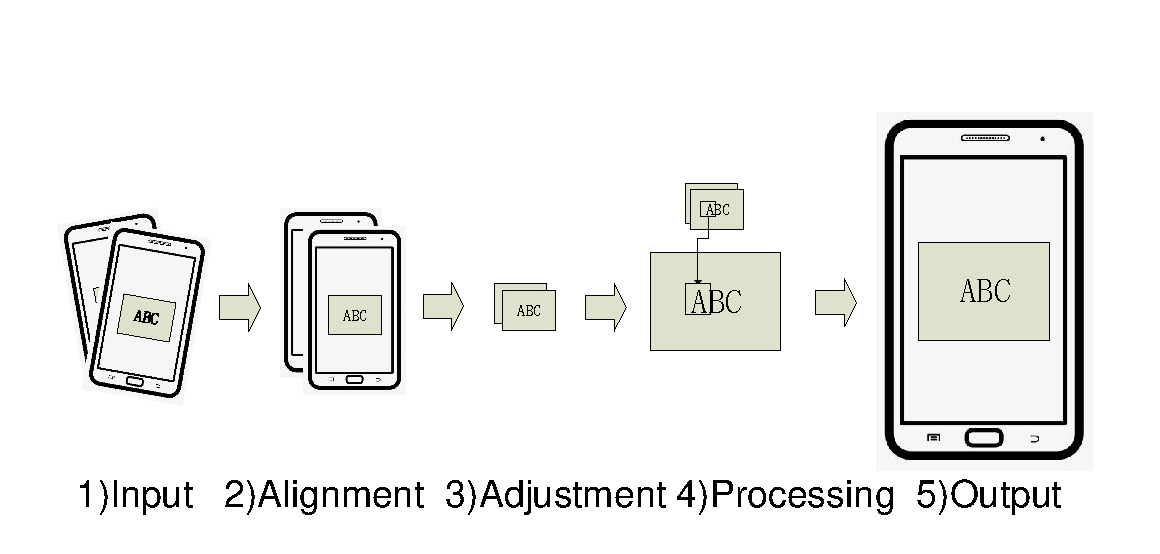
\includegraphics[width=0.5\textwidth]{./pic/workflow.pdf}
       \caption{Illustration of the workflow of our shoulder-surfing system.}
       \label{fig-workflow}
  \end{figure}
  \item \textbf{Model Complexity and adaption for variable input.} All the convolutional layers throughout the network are thus designed: They are performed individually for each image(or the featuremaps of them from the previous layer), and these convolutions in the same layer share a same set of parameters in training and production, thus reducing parameter count and avoiding convolutions for large numbers of channels, saving calculation power. This also leads to the benefit that the output featuremaps of all the images are the evaluations over the same set of features\cl{???}, so that the merging process can also be accomplished easily without the need of trainable parameters. In our design, the merging layers consists of simple pixelwize processes resembling average, min and max processors, to filter out either the collective or the most prominent features among the featuremaps. This process functions with any number of input images. As the convolutional processes are also performed individually for each layer, the same set of parameters of the network model can function normally with any number of input images, while the calculation complexity also increases linearly with the amount of input. On one hand, this gives our model the ability to adapt to the uncertainty of the number of avaliable images, providing relatively satisfactory results regardless whether the attacker has ample time photographing the target phone before it changes its display; on the other hand, the relative independence and the isotropy of the merging layers avoids the reliance on sequential order and consistency between neighboring frames(which is common among most multi-frame SR networks), solving the inconsistency problem mentioned in Figure~\ref{illustration_of_system}.
  \item \textbf{Compatibility with complex characters.} The discrete distribution of characters leads to the inclination of diviation and producing 'fake' results. The frequent introduction of input images is designed to mitigate this challenge. Also, our model is trained on these characters---the images we collected for the training dataset are all cropped so that only the characters remain, so that during the training processes the model can learn correlations between certain features and strokes, and the regular patterns of the characters, narrowing the possibilities offered by the blurry images. We also introduce adaptive boosting\cite{adaboost} in our training process, increasing the loss weight of the wrongly reconstructed characters, determined by loss in earlier stages and OCR in later stages, to accommodate the imbalanceness of data. The loss functions in training is also redesigned. The mean square error(MSE) is not suitable in this application, as a misplaced stroke, although highly obstructing readability, may only invoke a slight decrease in MSE because it only influenced a few pixels. Our solution is putting a weight on each pixel before applying weighted MSE. Assuming the characters are black on white, this weight increases at darker pixels and propagates to neighbouring dark pixels so that long strokes and intersections of strokes are given higher weights. This process serves as a supplement to MSE to focus more on readability and is beneficial for OCR and human reading tests. 
\end{itemize}



\section{System Design}
\label{sec-design}

\subsection{Design Principle}
To solve the challenges and outperform the state-of-the-art for this new shoulder surfing attack, we propose a holistic system with the multi-frame SR neural network, illustrated in Figure~\ref{fig-system}.
%\cl{These four parts are too long, try to whittle it away to half its length. Refer to the revised contents for challenges in Section introduction.}

\begin{itemize}[leftmargin=*]
    \item \textbf{Layered architecture and frequent introduction of input.} In our architecture all input images are processed simultaneously and separately, with the information from other images for reference, throughout the network. The initial input images are introduced into the dataflow at each layer, from beginning to end, forming a model with uneven depth, acting as an anchor for the reconstruction process so that the output will be faithful to truth from beginning to end, while preserving the deep mainstream of the model to be able to process such blurry images.
    \item \textbf{Merging layers to adapt multiple frames.} A merging process inside each layer functions as the revenue of communication across images integrates information from all the images into one, the result of which is then stacked with each image for the next convolution. At each layer the image is exposed to the consensuses of features from other images at the same level of complexity, acting as a verification for the hypothetical features extracted from the current image, so that in the training process more audacious features can be learned and proposed without fear of punishment from the final loss, increasing the quality of featuremaps throughout the network.
    \item \textbf{Inconsistency problem, model complexity, and adaption for variable input.} To counter the lack of consistency between frames, all the convolutional layers throughout the network are performed individually for each image with the same set of parameters. This not only reduces parameter count and calculation power, but also avoids reliance on consistency between neighboring frames. Furthermore, this allows variations in the number of input images.
    \item \textbf{Compatibility with complex characters.} The discrete distribution of characters leads to the inclination of deviation and producing 'fake' results. The frequent introduction of input images is designed to mitigate this challenge. Also, instead of using Mean Square Error(MSE) as the loss function, we put a weight on each pixel before applying weighted MSE. Assuming the characters are black on white, this weight increases at darker pixels and propagates to neighboring dark pixels so that long strokes and intersections of strokes are given higher weights. This process serves as a supplement to MSE to focus more on readability and is beneficial for OCR and human reading tests. 
  \end{itemize}

\subsection{Network Design}
The core of the \textsf{SRPeek} system is a specially designed multi-frame SR neural network, accepting a group of $N$ images indexed $x_1^{(0)}$ to $x_N^{(0)}$ as input and generating an image with higher resolution $y$ as output. The network comprises $L$ layers, each of which implements a non-linear transformation $H_l(\cdot)$, where $l$ indexes the layer. As mentioned before, in each layer images are processed separately, with the merging layers as revenue for communication, so that the output of each layer is correspondent to the input.  We denote the output of the $l^{th}$ layer as $x_1^{(l)}$ to $x_N^{(l)}$, which is also the input of the $(l+1)^{th}$ layer. Till now the model is not different from traditional SR models:
\begin{equation}\label{eq:1}
    \begin{split}
x_i^{(l)} = H_l(x_i^{(l-1)}), i=1,2,...N
\end{split}
\end{equation}

%\cl{function above cannot express merging between x1 x2 ... xN?}

Additionally, we introduce the initial images $x_i^{(0)}$ as an input for all the layers:
\begin{equation}\label{eq:2}
    \begin{split}
        x_i^{(l)} = H_l(x_i^{(l-1)},x_i^{(0)}), i=1,2,...N
\end{split}
\end{equation}

The last layer is exceptional, it yields a single image $y$ as output. 

Presently, in these layers nothing is done to raise the resolution of the images, so that the resolution of $x_i^{(0)}$ to $x_i^{(l-1)}$ and $y$ remains the same. To increase resolution, we insert several 2$\times$ nearest upsampling layers $U$ evenly throughout the architecture between the layers:
\begin{equation}\label{eq:3}
    \begin{split}
        x_i^{(l)} \leftarrow U(x_i^{(l)}), x_i^{(0)} \leftarrow U(x_i^{(0)}), i=1,2,...N
\end{split}
\end{equation}

we upsample the input images $x_i^{(0)}$ simultaneously to keep the two inputs of the following layers $H_l(x_i^{(l-1)},x_i^{(0)})$ unanimous in resolution. For example, in a 4$\times$ SR network with five layers, we may insert 2 2$\times$ nearest upsampling layers behind the 2nd and 4th layer.

Illustrated in Figure~\ref{fig-system}, inside each layer $H_l$ there are 3 convolution layers $Conv_{1l}(\cdot)$, $Conv_{2l}(\cdot)$, $Conv_{3l}(\cdot)$ and 1 merging layer $Merge_l(\cdot)$.

%\cl{$H(\cdot)$ or $H(\cdot,\cdot)$?}
\begin{figure}
    \centering
       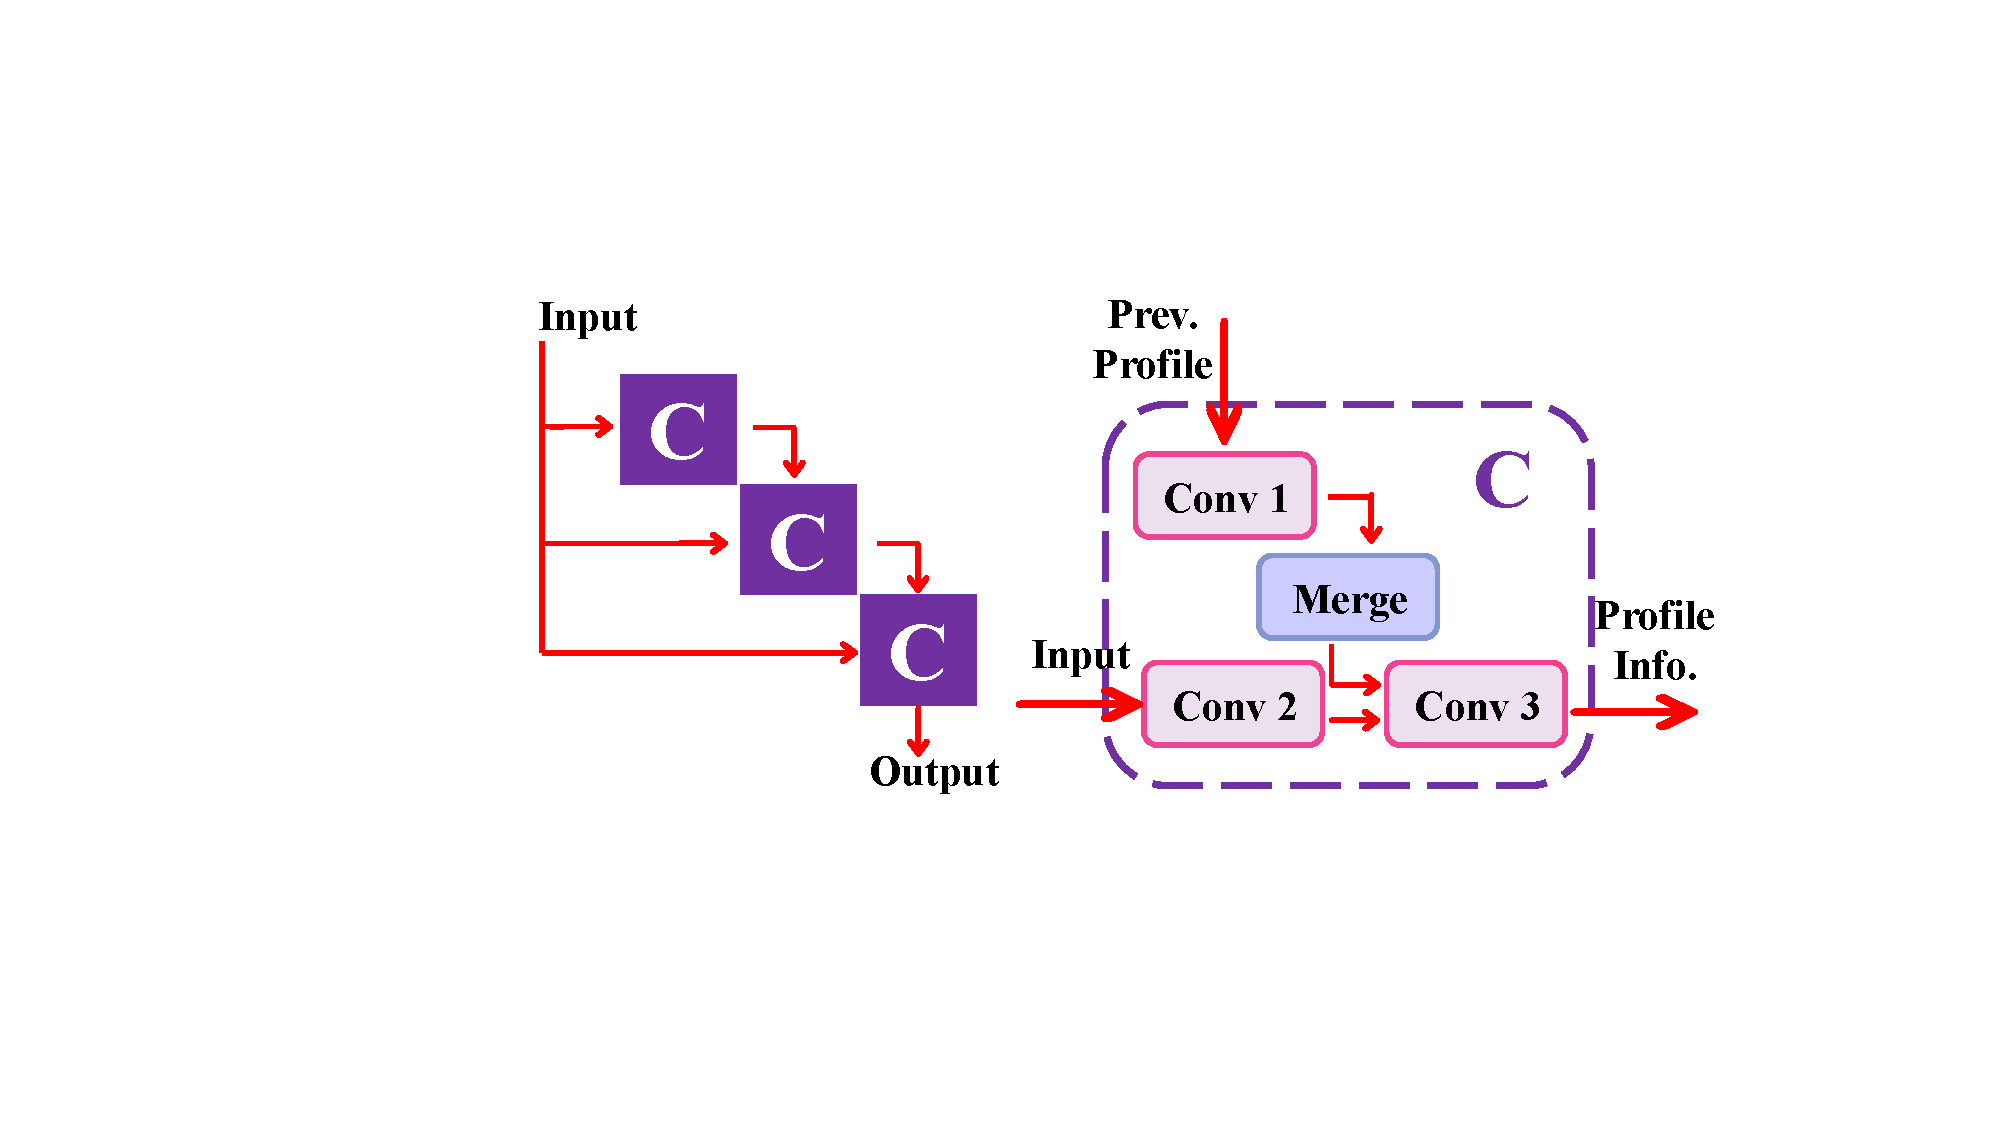
\includegraphics[width=0.90\linewidth]{./pic/network.pdf}
       \caption{Core network architecture of SRPeek.}
       \label{fig-system}
   \end{figure}   

\vspace{1mm}
\noindent
\textbf{Conv1:} The first convolutional layer, $Conv1$, accepts the layer's first input parameter $x_i^{(l-1)}$ as input. Note that all three convolutional layers accept a single image (or its featuremaps from the last convolutional layer) as input, the convolutional process is repeated for all the images, and calculations within the same convolutional layer share the same group of parameters all the time (parameters denoted as $Param_{sl}$ for convolutional layer $Conv_{sl}, s=1,2,3$):
\begin{equation}\label{eq:4}
    \begin{split}
        a_i^{(l)} = Conv_{1l}(x_i^{(l-1)},Param_{1l}), i=1,2,...N
\end{split}
\end{equation}

\vspace{1mm}
\noindent
\textbf{Merge:} The results of the previous step of all the images $\{a_1^{(l)},a_2^{(l)},...,a_n^{(l)}\}$ are then passed to the merging layer $Merge_l$ to generate $t$ groups of featuremaps. Suppose the results of $Conv_{1l}$ consists of $R$ channels:
\begin{equation}\label{eq:5}
    \begin{split}
        a_i^{(l)} = \{a_{i1}^{(l)},a_{i2}^{(l)},...,a_{iR}^{(l)}\}, i=1,2,...N
\end{split}
\end{equation}

The data in each channel will be merged separately in the merging layer. The output is $T\times R$ channels, denoted as $b_{tr}^{(l)}(t=1,2,...T, r=1,2,...R)$:

\begin{equation}\label{eq:6}
    \begin{split}
        b_{tr(p,q)}^{(l)} = \sum_{i=1}^{N} a_{ir(p,q)}^{(l)} e^{k_t a_{ir(p,q)}^{(l)}} /\sum e^{k_t a_{ir(p,q)}^{(l)}}
\end{split}
\end{equation}

where (p,q) represents the pixel at this coordinate, and $k_t$ is a set of fixed parameters shared in all the merging layers throughout the model, controlling the behavior of the merging process. Apparently, k=0 leads to averaging, k=${+\infty}$ leads to max operator and k=${-\infty}$ leads to min operator. We use T=5 and k=-1,-0.5,0,0.5,1 in our model, giving consideration to both consensuses (k=0,averaging) and prominent features(k=1, 'soft'max and k=-1, 'soft'min). these $T\times R$ channels $b_{tr}^{(l)}$ is the output of this merging layer $Merge_l$.

\vspace{1mm}
\noindent
\textbf{Conv2:} $Conv2$ is a replica of $Conv1$, processing the layer's second input parameter $x_i^{(0)}$, also generating $N$ outputs with $R$ channels per output, denoted as $c_ir^{(l)}, i=1,2,...N, r=1,2,...R$:
\begin{equation}\label{eq:7}
    \begin{split}
        c_i^{(l)} &= Conv_{2l}(x_i^{(0)},Param_{2l}), i=1,2,...N\\
        c_i^{(l)} &= \{c_{i1}^{(l)},c_{i2}^{(l)},...,c_{iR}^{(l)}\}, i=1,2,...N\\
\end{split}
\end{equation}

\vspace{1mm}
\noindent
\textbf{Conv3:} The data from $Merge$ and $Conv2$ are merged together, in that all the $T\times R$ channels of $b_{tr}^{(l)}$ are replicated N times and stacked with each one of the N outputs of $Conv_{2l}$, before these N outputs, each with $(T+1)\times R$ channels, are passed through the third convolutional layer $Conv_{3l}$. There are also N output of this convolutional layer, denoted as $d_i^{(l)}, i=1,2,...N$:
\begin{equation}\label{eq:8}
    \begin{split}
        d_i^{(l)} = Conv_{3l}(Stack(c_i^{(l)},b^{(l)}),Param_{3l}), i=1,2,...N 
\end{split}
\end{equation}

\vspace{1mm}
\noindent
\textbf{Output:} If $l < L$, this is not the last layer, the N outputs of step (4) will be the output of layer $H_l$. Otherwise, as we need to present a single image $y$ as output, we add another merging and a common convolutional layer after $Conv_{3l}$. The merging layer is identical to the previous $Merge_l$, merging the N outputs $d_i^{(l)}$ into $T\times R$ channels $e_{tr}^{(l)}$, and a convolutional layer processes this $e_{tr}^{(l)}$ to generate a single channel of output $y$. 
\begin{equation}\label{eq:7}
    \begin{split}
        \{e_{tr}^{(L)},t\le T,r\le R\} &= Merge'_{L}(\{d_i^{(L)},i\le N\})\\
        y &= Conv'_{L}(\{e_{tr}^{(L)},t\le T,r\le R\} )\\
\end{split}
\end{equation}

% \subsection{Design Principal}
% To solve the challenges and outperform the state-of-the-arts for this new shoulder surfing attack, we propose a holistic system with the multi-frame SR neural network, illustrated in Figure~\ref{fig-workflow}.
% \cl{These four parts are too long, try to whittle it away to half its length. Refer to the revised contents for challenges in Section introduction.}

% \subsection{system design}
% We implemented a holistic system for shoulder surfing, with the neural network as core, on a smartphone to verify the efficiency of our model. It iterates through the following steps: 

% \vspace{1mm}
% \noindent
% \textbf{Input:} Under guidance of the attacker, The smartphone will zoom in, take focus, and take 20 images with burst mode of the target screen. Note that the zoom in step is only for easier interaction and focusing, and to utilize the telephoto lenses and optical zoom, if available, as digital zooming do not put in any extra data; On traditional phones with only digital zooming, the photo-taking will be with 1x zoom, and on phones with optical zooming, 5x to 10x zoom, depending on the optical zooming range. This way information on the images will be more compact and easier to comprehend by neural networks.

% \vspace{1mm}
% \noindent
% \textbf{Alignment:} The images are then aligned to mitigate the shifts between frames caused by hand tremor or movements from the lenses, as cameras with optical lenses will occasionally shift slightly across time due to the movements of its inner mechanism. Luckily, in our scenario the target is a glowing screen whose edges are easily distinguishable in most cases, and we use them as reference to align our images. The images are also spun to make the text horizontal in the process. The screen is cropped out and the rest of the image abandoned.


% \vspace{1mm}
% \noindent
% \textbf{Adjustment:} The lines of text(or stuff differing from the background color of the screen) will be carved out for processing, to reduce the workload of the network. The characters are normally around 10x10 pixels in the photos, and the carved segments will leave 2 pixels of padding on all sides to avoid mutilating the character; A certain amount of error is allowed, but if the size of the text is too small or too large, the neural network will not be able to extract features normally, so the images will be zoomed to the right size(and the zooming of step (1) will be adjusted accordingly).


% \vspace{1mm}
% \noindent
% \textbf{Processing:} As our network accepts only 9x9 patches, we will process all the 9x9 patches among the input photo and merge the results together. After carving a 9x9 patch at corresponding locations of each image, these patches are then processed by our multi-frame super resolution network, generating a single 36x36 image (4x upscaling). The input is RGB colored, while the output, as we are not interested in color, is black and white. When all patches are processed, their outputs are merged together. The overlapping pixels are thus processed: among all the outputs containing this pixel, we collect these values, remove outliers, and use their average as the result. In this way, we generate upscaled image segments of all the characters on the target screen, which are then inserted in one of the input images (roughly upscaled to encompass them, just for reference) and displayed to the attacker.

% These steps are repeatedly executed to enable the attacker to monitor the victim at an interval of a few seconds. At critical times requiring continuous monitoring so as not to miss transient display, e.g. password entering, the system can simply lengthen the input phase across that period and process the data afterwards. The workflow of our system is shown in Figure~\ref{fig-workflow}.




\section{Implementation \& Training}
\label{sec-implementation-and-training}

\subsection{Data Collection}
\label{sec-experiment-setting}

In our experiment, we are forced to collect the training dataset on our own instead of using public datasets. Because of our unique application, to the best of our knowledge there is no publicly available image dataset built for shoulder-surfing. Modern network architectures work with naturally obtained images, e.g. ordinary photos, satellite images, scanned documents, YouTube videos, etc. where the images are well focused and captured within the imaging ability of the camera, with the objects of interest, e.g. the face or the printed word, at least visible to the naked eye. and we apply the SR algorithms to reduce noise and refine details, like repainting texture and refining edges. However, as emphasized above, in our application we face images that is extremely blurred and distorted, due to the extreme circumstances when the photos are taken, and it is impossible to tell from each single picture whether a stroke of a character really belongs here, as it's equally possible that this line is a distorted mixture of multiple lines or is a mutilated part of a longer stroke. These are the reasons why our work does not choose datasets that are publicly available, and collect data by ourselves--as it will completely defeat the purpose if we turn to these datasets. And this also explains why we failed in trying to get comparable results with other SR architectures we use as baselines, as these networks are designed for another purpose and they hardly ever faced such distorted and blurred images.

The task of data collection is quite tedious, as we discovered that we need photos taken in all kinds of environments to train a robust network. We initially collect 60,000 images with the position of the smartphones static and all other environmental parameters stationary, and divided it into training and testing datasets which do not have common characters between them. Note that different lenses have different photographing abilities and blurring patterns, so the model has to be trained for each phone model. When using smartphones with optical zoom, the images will shift slightly time after time even if we keep them completely still, so the aligning phases are still needed (this shifting is also beneficial in that it simulates normal hand tremors in real-life scenarios even if we fix the phone to a stand instead of holding it up throughout the data collection phase which can last several hours). There are no consistency between adjacent images, so we also shuffle the images to increase this shifting effect and increase the variety of the training data. %To reduce calculation and better align the images with the ground truth, in the training data collection phase we drew a box around the text on the victim's screen, replacing the edges of the phone for alignment and cropping in the alignment step (as shown in Figure~\ref{fig-training}), but our system works perfectly without it.

Our network easily learned the patterns and presented equally satisfactory results in the test dataset (see Figure~\ref{fig-train-single-2}), displaying clean, easy to read results, showing that the network has learned to extract features beneath the character level, and it is highly possible that this network can recover all kinds of characters, not limited to the characters in the training dataset. However, when we slightly modified the environment, the images displaying the text with a different shade and size, none of the features were successfully extracted, and the network outputted white noise (see Figure~\ref{fig-train-single-4}).
 \begin{figure}
     \centering
     \subfigure[input from same environment]{
         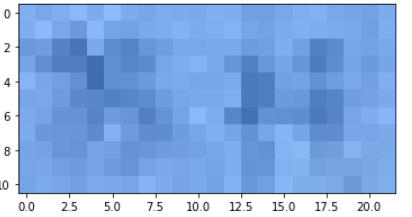
\includegraphics[width=0.2\textwidth]{pic/training_single_dataset_1.png}
         \label{fig-train-single-1}
         }
     \subfigure[output of (a)]{
         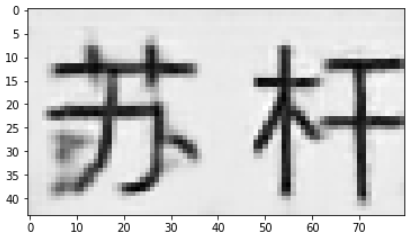
\includegraphics[width=0.2\textwidth]{pic/training_single_dataset_2.png}
         \label{fig-train-single-2}
         }
     \subfigure[input from different environment]{
         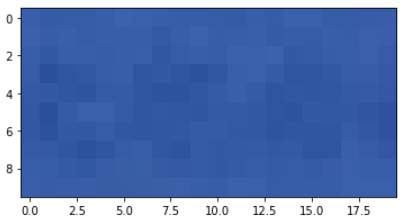
\includegraphics[width=0.2\textwidth]{pic/training_single_dataset_5.png}
         \label{fig-train-single-3}
         }
     \subfigure[output of (c)]{
         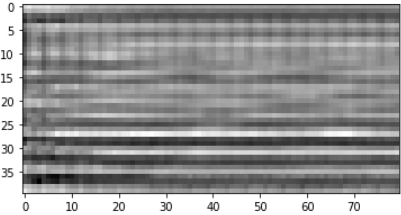
\includegraphics[width=0.2\textwidth]{pic/training_single_dataset_4.png}
         \label{fig-train-single-4}
         }
    % \subfigure[ground truth]{
     %    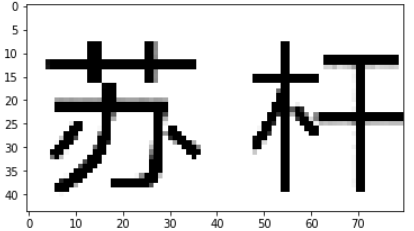
\includegraphics[width=0.2\textwidth]{pic/training_single_dataset_3.png}
      %   \label{fig-train-single-5}
       %  }
        \caption{Results of training with data collected in fixed environment. The network performs well in this environment but fails in other.}
        \label{fig-train-single}
\end{figure}

\subsection{Experiment Setting}
As a result of these observations, we have to collect images in varied environments. Our experiment consists of 2 smartphones, one for the attacker and one the victim. Their distance is between 1 and 2 meters for traditional lenses(for the camera of the attacker's phone) without optical zooming, and 5 to 7.5 meters for lenses with optical zooming. Both phones are fixed to stands to keep them completely still, but as mentioned above, the lenses with optical zoom will shift slightly time to time, which is similar to a handheld situation. An app runs inside the attacker's phone, taking photos continuously, adjusting its focus and aperture, trying it's best to capture high-quality photos. Another app runs inside the victim's phone, displaying random characters with several fonts and colors, for the attacker to capture. The characters are selected from commonly used Chinese characters with 5 to 10 strokes and the English alphabet, and we divide this assemble into training and testing subsets. As the English characters are apparently easier to classify and reconstruct for the networks, the experiments testing the performance of the network will be performed only on Chinese characters, but it is our observation that our system works on English characters as well as Chinese characters.

As the experiment goes on, the attacker phone will keep on taking photos in burst mode (20 photos per time), and the victim phone will change the characters it is displaying at a fixed interval, when approximately 100 images were taken by the attacker. We change the environmental setting whenever about 2k photos were taken, relocating the phones (while keeping their distance between 1 and 2 meters) or modifying the angle of the phones. The attacker will always point its phone directly at the victim, keeping its screen in the middle of the photos; The victim, however, may tilt its phone at an angle within 30 degrees. We then readjust the focus and aperture of the attacker's phone to maximize the image quality before continuing data collection. Screenshots were taken in the victim's phone each time it changes its display, and these screenshots are scaled, spun and deformed according to the distance and angle between the phones at the time, and used as ground truth for training and evaluation.
\begin{figure}
	\centering
	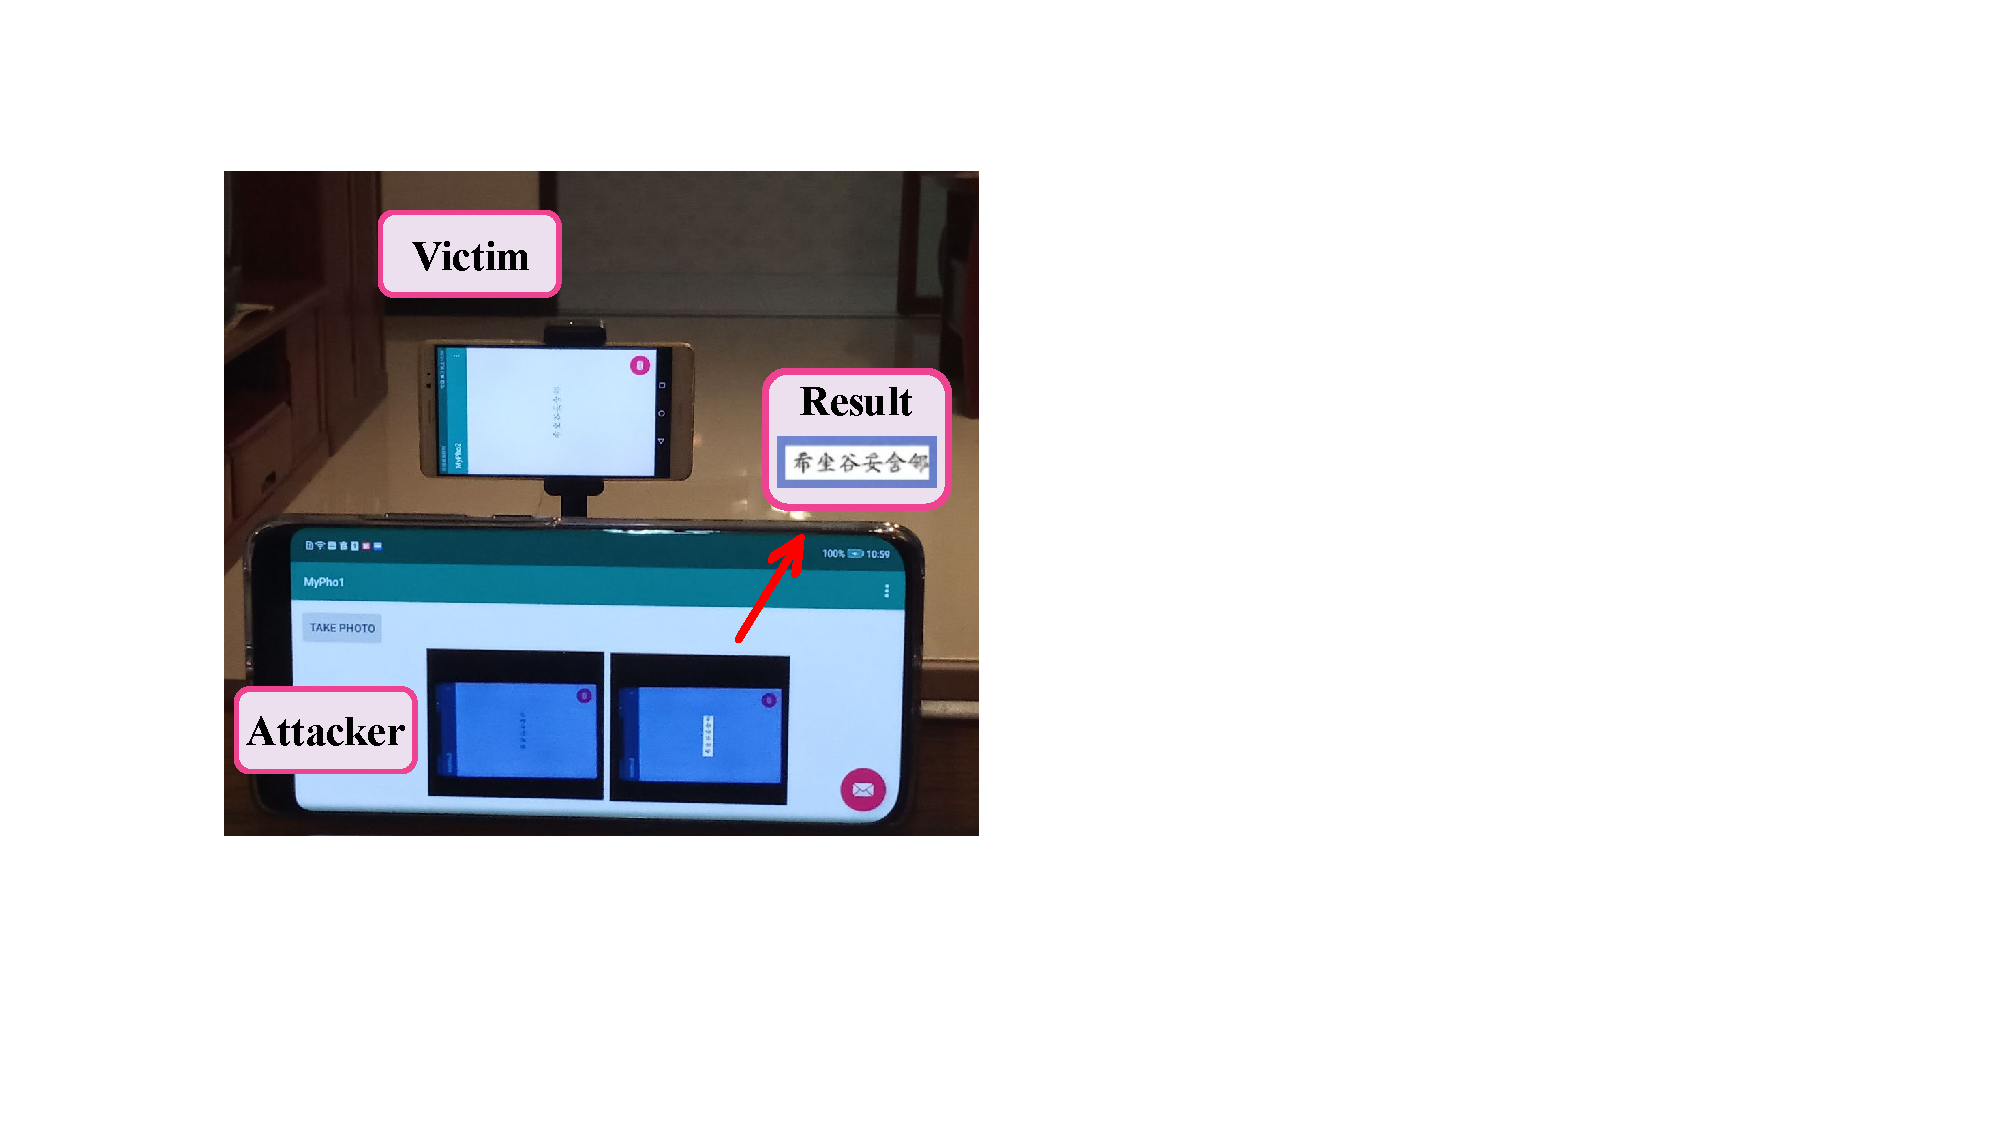
\includegraphics[width=0.48\textwidth]{pic/setup.pdf}
    \caption{Illustration of our experimental setting (Distance between phones are shortened for demonstration).}
	\label{illustration_of_system}
\end{figure}
% \begin{figure}
%   \centering
%      \centering
%      \subfigure[Experiment setting. Distance between phones are shortened for demonstration.]{
%          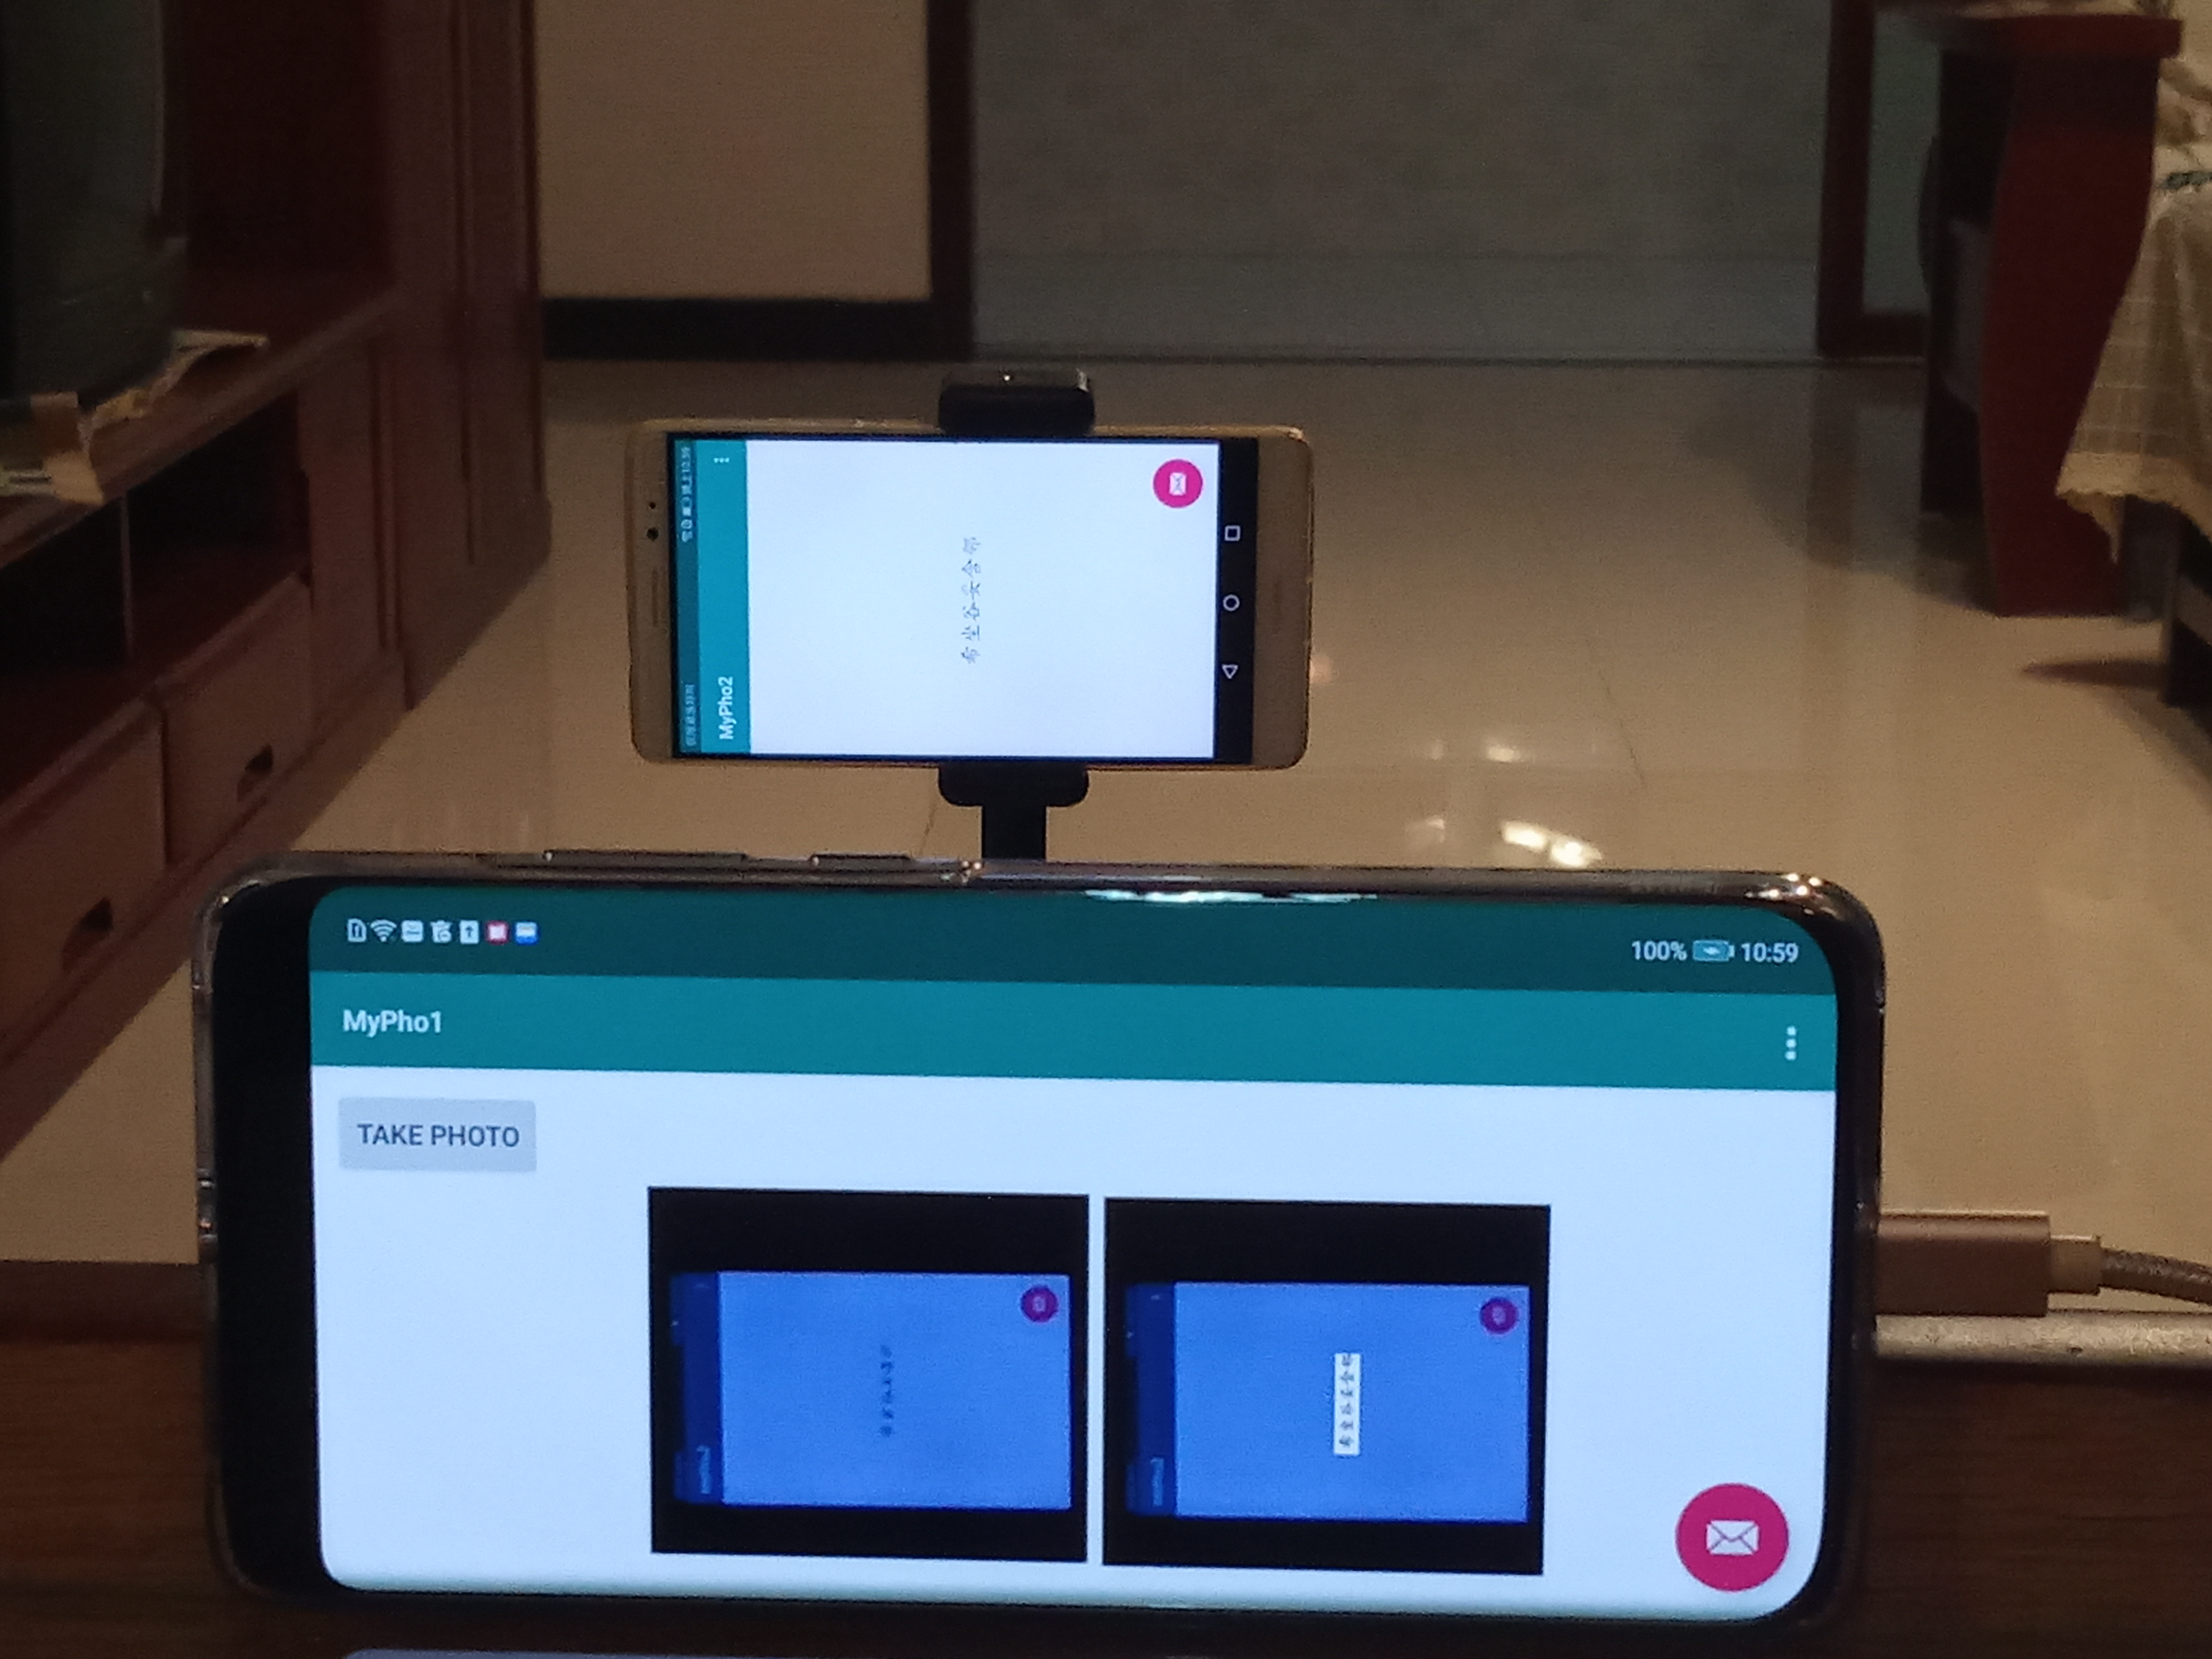
\includegraphics[width=0.5\textwidth]{pic/exp1.jpg}
%          \label{fig-exp1}
%          }
%    \subfigure[screenshot from attacker's phone(SRPeek system).]{
%          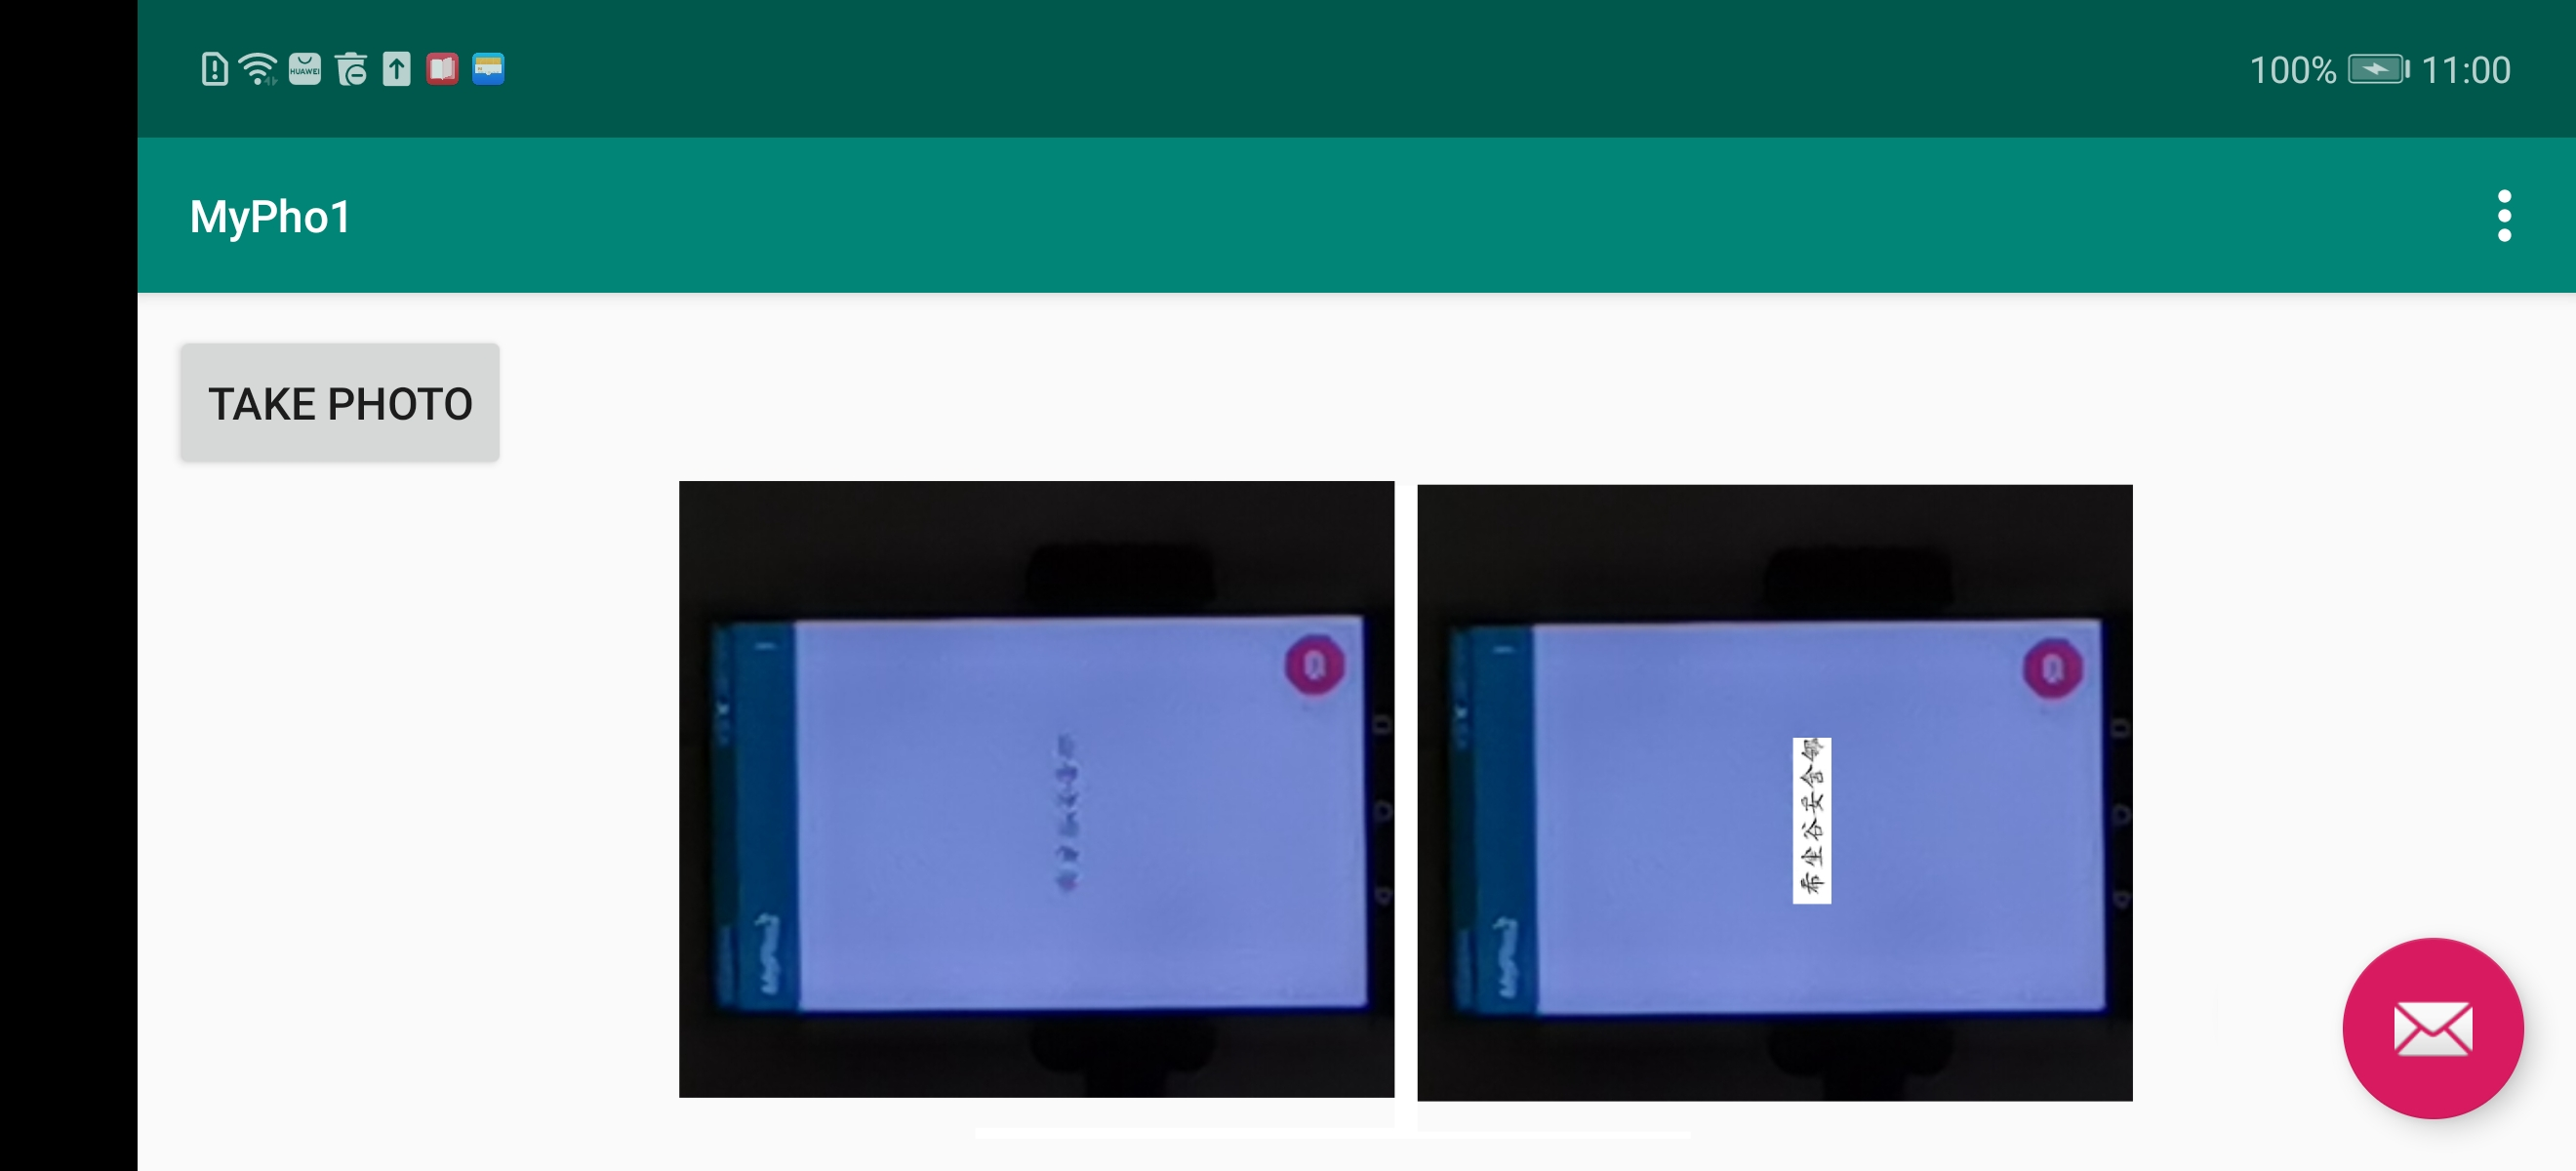
\includegraphics[width=0.5\textwidth]{pic/exp2.jpg}
%          \label{fig-exp2}
%          }
%    \subfigure[screenshot from victim's phone.]{
%          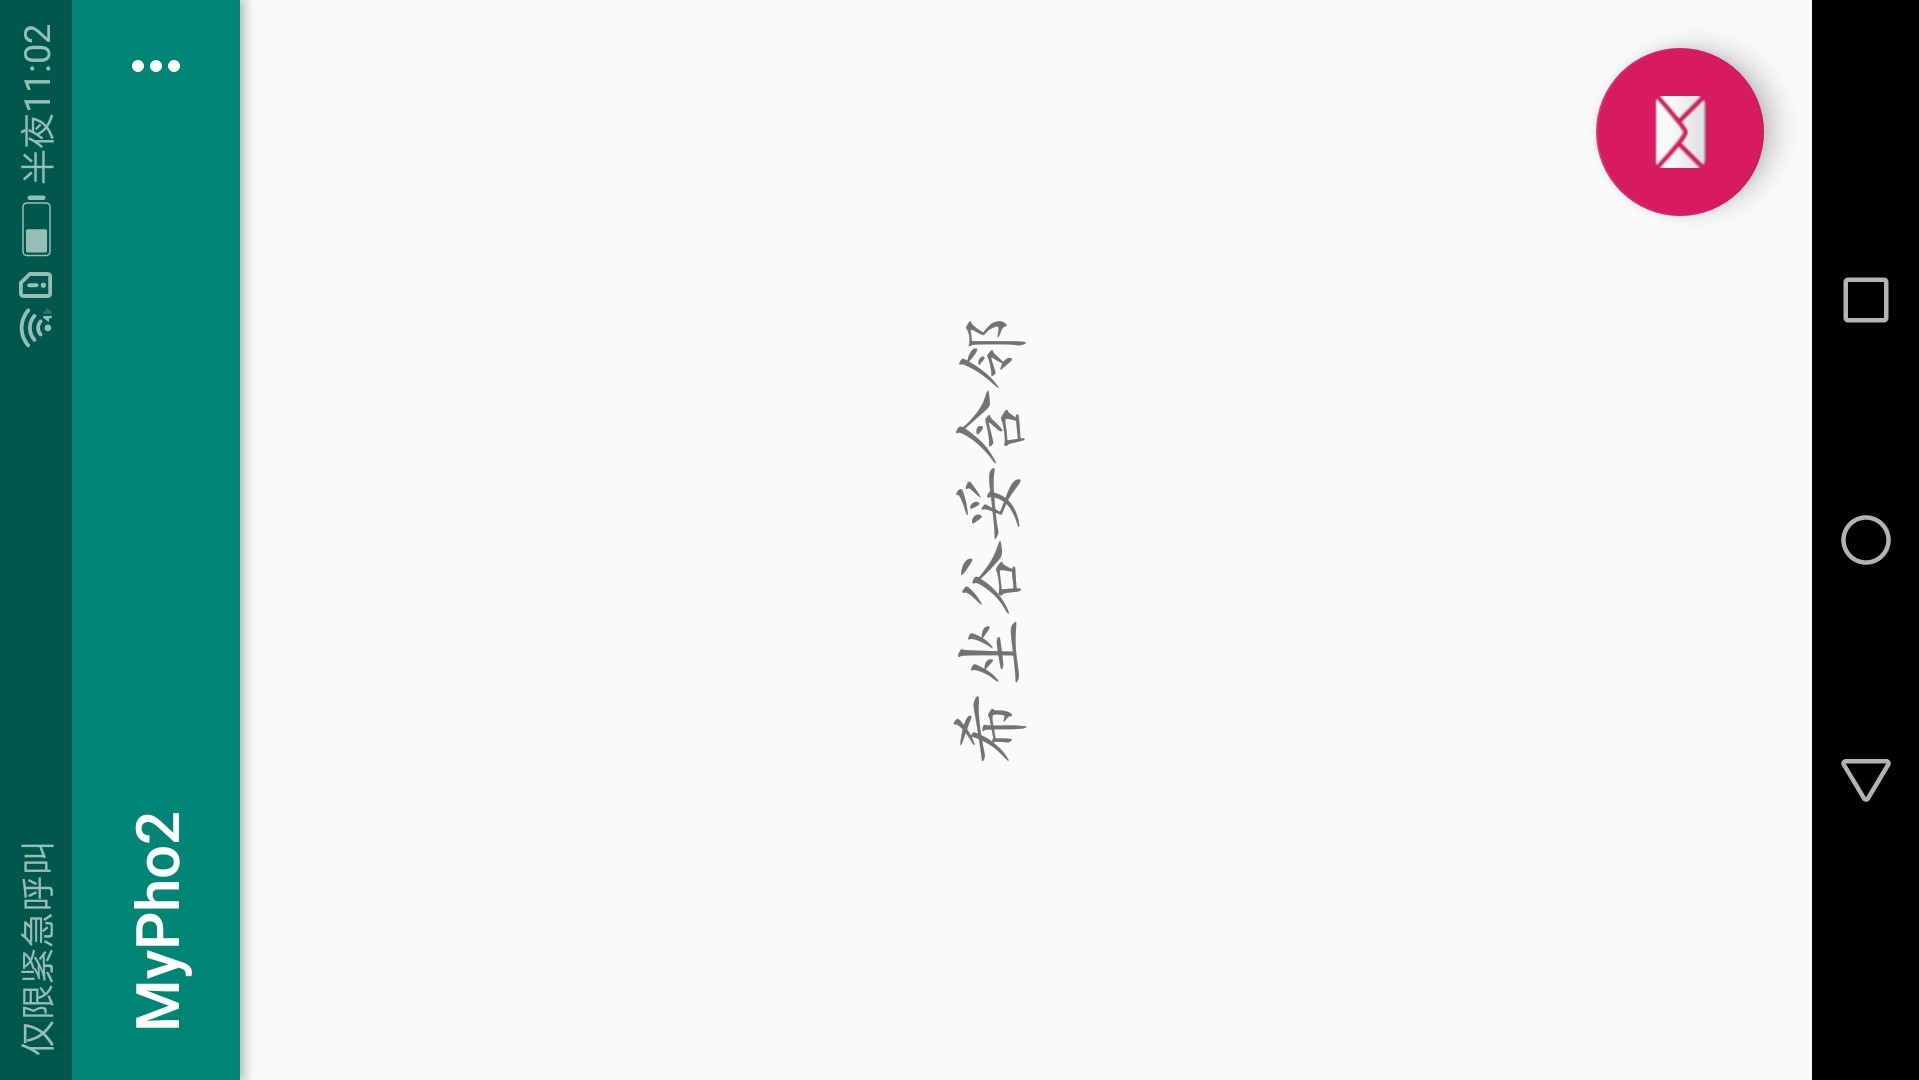
\includegraphics[width=0.5\textwidth]{pic/exp3.jpg}
%          \label{fig-exp3}
%          }
%      \caption{Illustration of our experimental setting.}
%      \label{fig-experiment}
% \end{figure}

The data was collected indoors, as is often the case of shoulder-surfing in public areas (theaters, subways, offices, etc.). We perform the experiment in a room with a window and repeat the data collection phase in different times of the day and night, with curtains drawn or open, lights turned on and off to modify the illumination parameter. The position of the phones is also a crucial factor in this parameter, and we avoid extreme settings, e.g. having the sunlight directly shining on the screen. We collected 800,000 images in this way with a Redmi6A phone (which possess a camera with 130 million pixels). This process is extremely time-consuming, but the data amount is crucial in our experiment, as slight variations of the environment will cause drastic changes in the features extracted from the characters, and only by covering the variations in each of the environmental parameters in the training data can the system successfully function in different scenarios.

\subsection{Model Specifications}
It is our observation that cameras in different phones display different patterns of distortion when performing the shoulder-surfing experiment, and apparently, images captured from a phone with weaker abilities (less pixels, less range of focus, worn lenses, etc.) will need a stronger, more complex model to extract the features. Thus, the specifications of our model are only for reference and may not work when reproduced on another phone.

Our model accepts 20 images at a time, with a size of 9x9 pixels. The model consists of 5 blocks described in the previous section. In each block, feature maps from the previous layer are passed through a single convolutional layer with 32 channels of feature maps as output. the 20x32 feature maps are then merged horizontally with the max-min-average process, and the output is 5x32 channels. Simultaneously, the original input images are processed again with a single convolutional layer with 32 channels output, and stacked with the former 5x32 channels to form a dataflow of 6x32 channels for each one of the 20 images. These channels are finally passed through a single convolutional layer, outputting 32 channels per image for the next block. The kernels in each convolutional layer is 3x3. We also insert LeakyReLU and Batch Normalization processes after each convolutional layer, and 2 upsampling layers between the 5 blocks. A single 1x1 convolutional layer is placed after the 5 blocks with a single channel as output to form the final output layer. This model consists of approximately 200,000 parameters and a complexity of about 400,000 FLOPs. As a light-weighted model, it makes a prediction within 0.1 seconds on a Tesla K80 GPU over a 9x9 patch, and when implemented on a smartphone, the human user can recognize a character within 2 seconds of processing time.

\subsection{Training Process}
Because of the difficulties in discovering the patterns among the blurry images, the training process is not so straightforward and somewhat time-consuming. Our approach is as follows: we first collect 60,000 images at a stationary experiment setting and train the model with it, as mentioned in Sec~\ref{sec-experiment-setting}, until we get satisfactory results on the test dataset. The model should be able to handle this task easily. After that, we use transfer learning methods to fine tune the model in order to fit different environmental parameters. We add a small percentage of image data from another similar experiment setting into the training data and resume training. When the model stabilizes, continue adding data from the same setting until the model can equally process data from the two image collections. Note that in this process the model will tend to extract false features, displaying wrong but clear texts as result. This phenomenon can be mitigated with dropout and normalization layers. As the model successfully fits two of the image sets, we repeat this procedure for several times until it shows signs of self-adapting, for example, when presented photos taken at 1.8m and 1.2m range in the training process, the model fits 1.5m photos easily. After that, the model can learn with the full fully-shuffled dataset with fewer difficulties.


\section{Model Evaluation}
\label{sec-evaluation}
% \begin{figure*}[!t]
%     \centering
%     \subfigure[Traditional Lens]{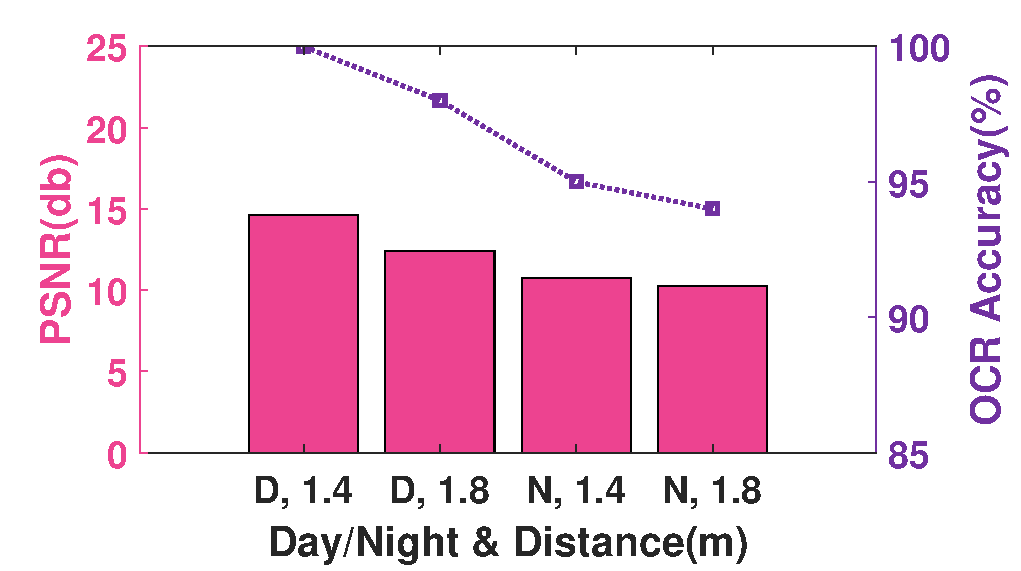
\includegraphics[width=0.24\textwidth]{./pic/data_1.pdf}\label{fig-control-1}}
%     \subfigure[Optical Lens]{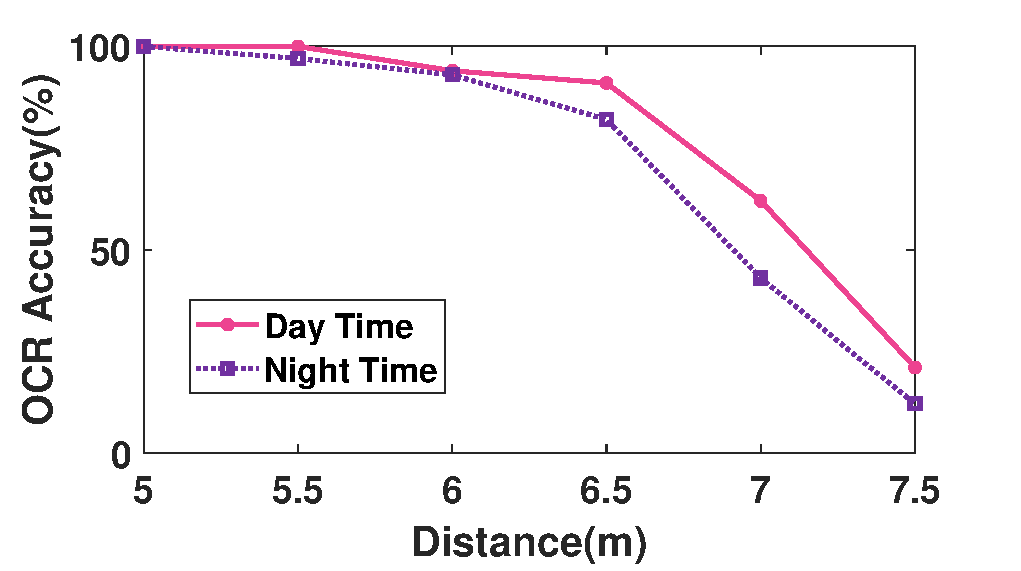
\includegraphics[width=0.24\textwidth]{./pic/data_1_2.pdf}\label{fig-control-2}}
%     \subfigure[Traditional Lens]{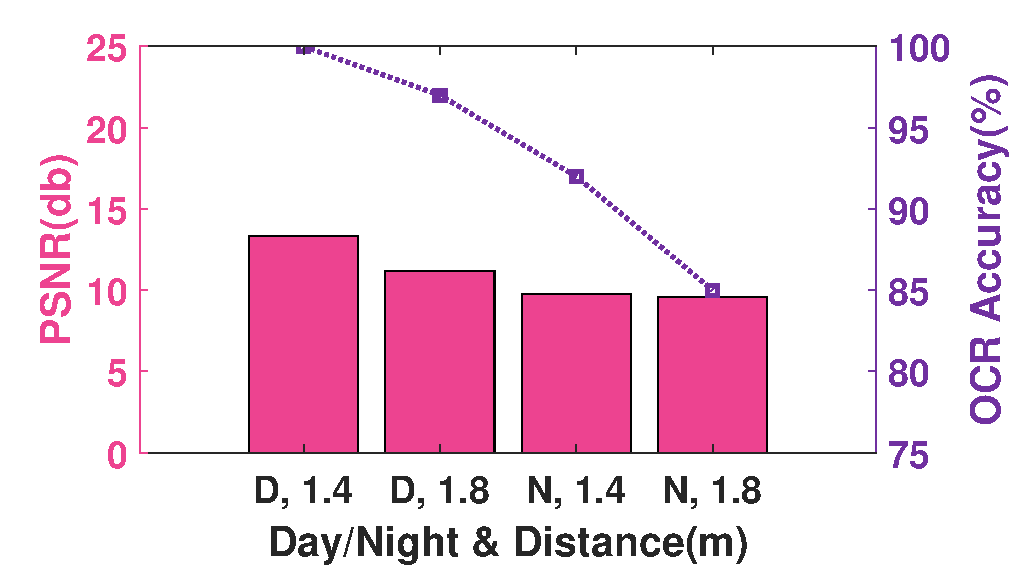
\includegraphics[width=0.24\textwidth]{./pic/data_2.pdf}\label{fig-random-1}}
%     \subfigure[Optical Lens]{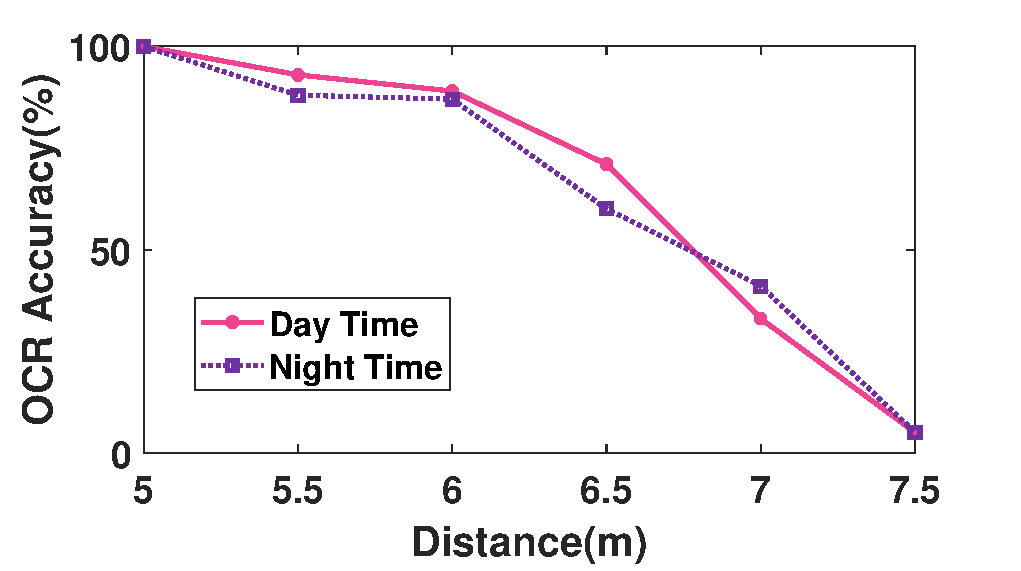
\includegraphics[width=0.24\textwidth]{./pic/data_2_2.pdf}\label{fig-random-2}}
%     \hfill
%     \caption{Performance in Controlled Environment (a,b) and Random Environment (c,d).}
%     \label{fig-performance-1}
% \end{figure*}
We evaluate the performance of the network model in different training and testing conditions. We perform the following experiments with two Custom Off-The-Shelf(COTS) smartphones: a Redmi 6A smartphone, with a single rear camera with 13 million pixels and digital zoom only, and a HUAWEI P40 Pro, with multiple rear cameras. The telephoto camera possess up to 5x optical zooming ability which we will utilize fully in our experiments.
 
\subsection{Performance In Controlled Environments}
% \begin{figure}[!t]
%     \centering
%     \subfigure[Traditional Lens]{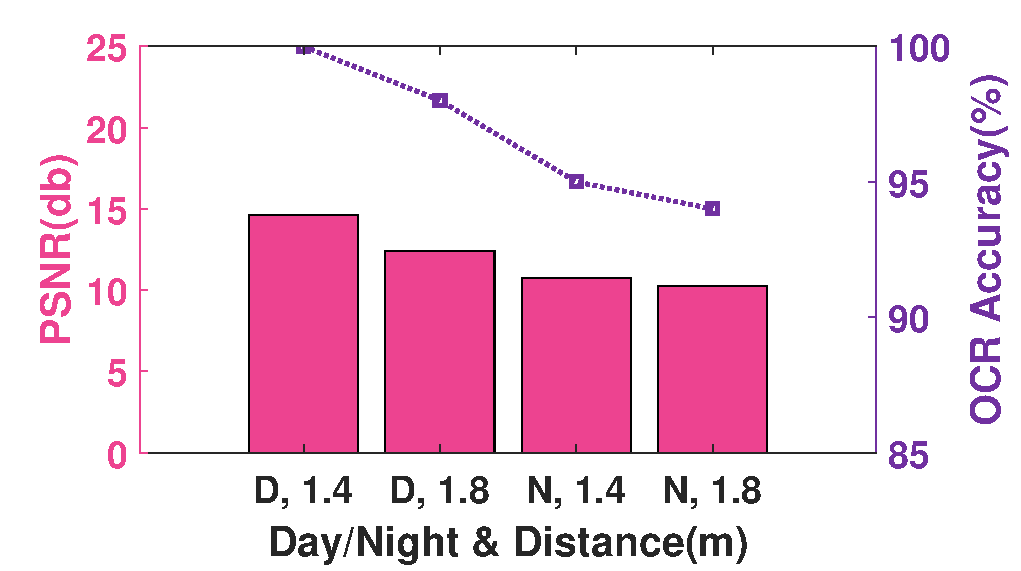
\includegraphics[width=0.40\textwidth]{./pic/data_1.pdf}\label{fig-control-1}}
%     \subfigure[Optical Lens]{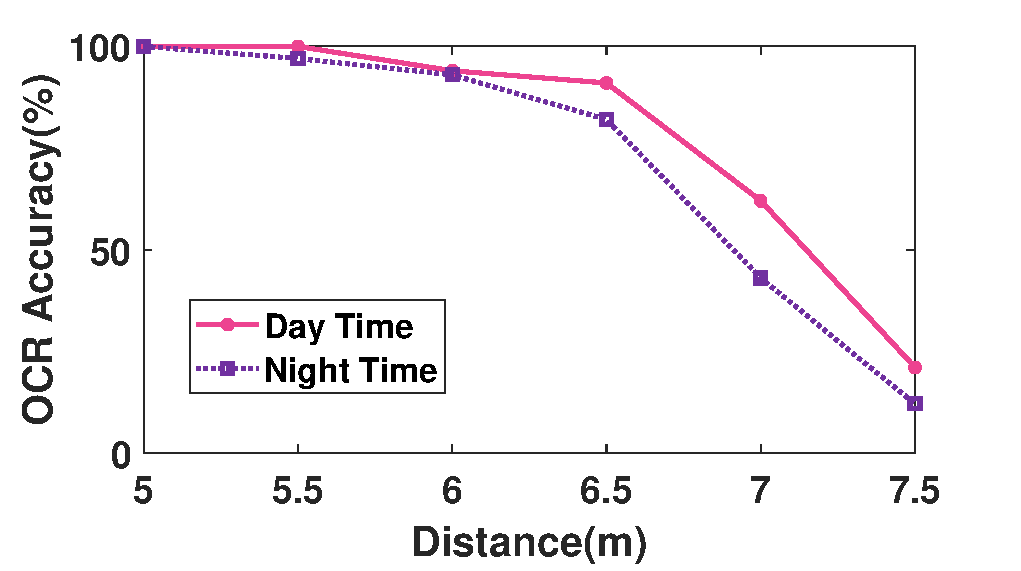
\includegraphics[width=0.40\textwidth]{./pic/data_1_2.pdf}\label{fig-control-2}}
%     \hfill
%     \caption{Performance in the controlled environment using traditional lens and optical lens.}
%     \label{fig:control}
% \end{figure}

In these experiments, we train and test the model with the images captured with exactly the same environment parameters, and used Peak Signal to Noise Ratio(PSNR) to evaluate the accuracy of the recovered images. The results are shown in Figure~\ref{fig-control-1} and Figure~\ref{fig-control-2}. Optical Character Recognition (OCR) services are also utilized to evaluate the accuracy. The traditional lens group is trained and tested at 1-2 meters distance, while the optical lens, 5-7.5 meters, where less than 5\% of the characters can be read with the naked eye. The PSNR and OCR results are shown in Fig. ~\ref{fig-control-1}.

This model can achieve an OCR accuracy above 90\% at 1.8m with traditional lens and at 6m with optical lens. Performances are relatively consistent in both day and night time, while increased distances mean less data, causing more artifacts(missing or misplaced strokes, etc.). It is the nature of Chinese characters that one mistaken stroke will largely affect its readability, leading to the result that while the pixel-wise error rises steadily with the increased distance, the accuracy will experience a drastic drop.

\subsection{Performance In Random Environments}
We train the model with data captured in different environments, as mentioned before, and test its ability in other environments. The results are shown in Figure~\ref{fig-random-1} and Figure~\ref{fig-random-2}. We can observe that the model performs best in daytime and at closer distances. For Figure~\ref{fig-random-1}, the model can still achieve an OCR accuracy above 85\% at 1.8m with traditional lens. From Figure~\ref{fig-random-2}, the OCR accuracy keeps higher than 90\% at 6m with optical lens. This verifies the efficiency of our model for environment adaption.

% \begin{figure}[!t]
%     \centering
%     \subfigure[Traditional Lens]{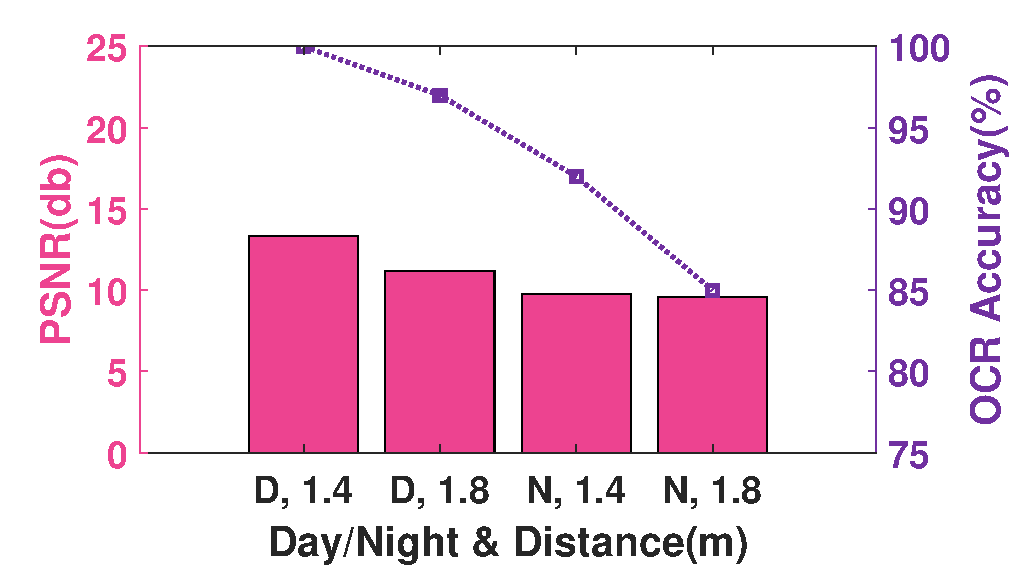
\includegraphics[width=0.40\textwidth]{./pic/data_2.pdf}\label{fig-random-1}}
%     \subfigure[Optical Lens]{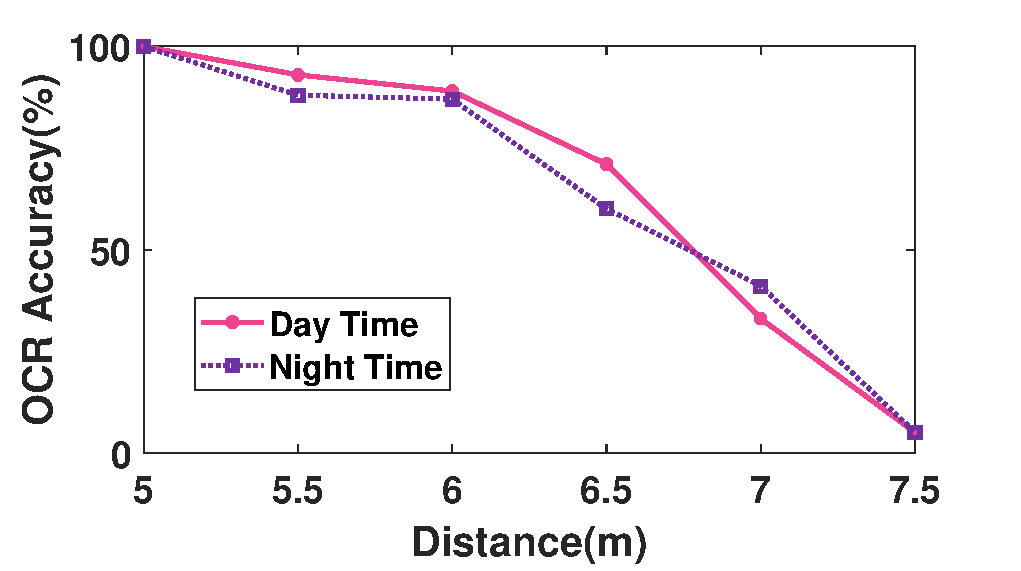
\includegraphics[width=0.40\textwidth]{./pic/data_2_2.pdf}\label{fig-random-2}}
%     \hfill
%     \caption{Performance in the random environment using traditional lens and optical Lens.}
%     \label{fig:control}
% \end{figure}

\begin{figure*}[!t]
    \centering
    \subfigure[Traditional Lens]{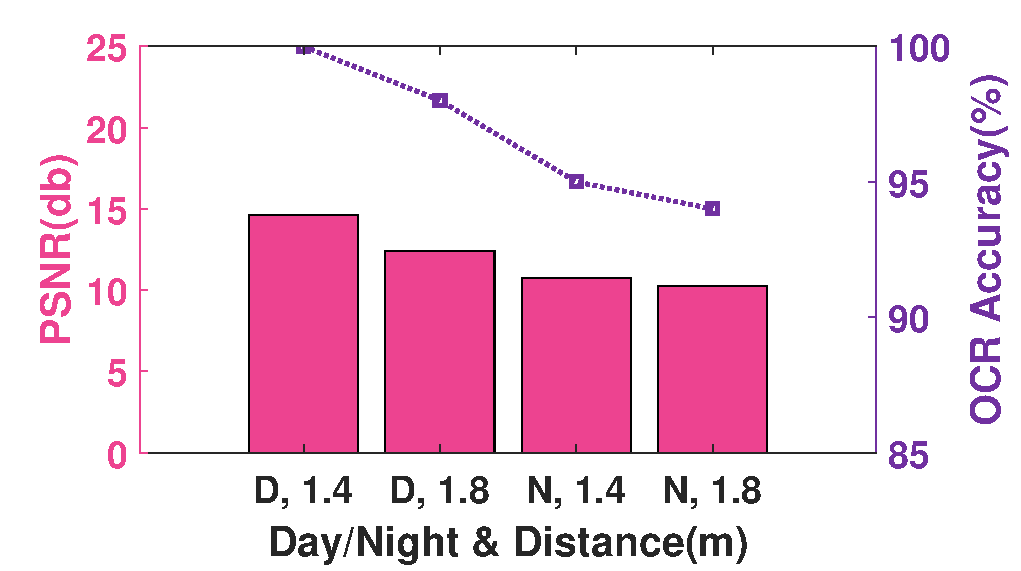
\includegraphics[width=0.24\textwidth]{./pic/data_1.pdf}\label{fig-control-1}}
    \subfigure[Optical Lens]{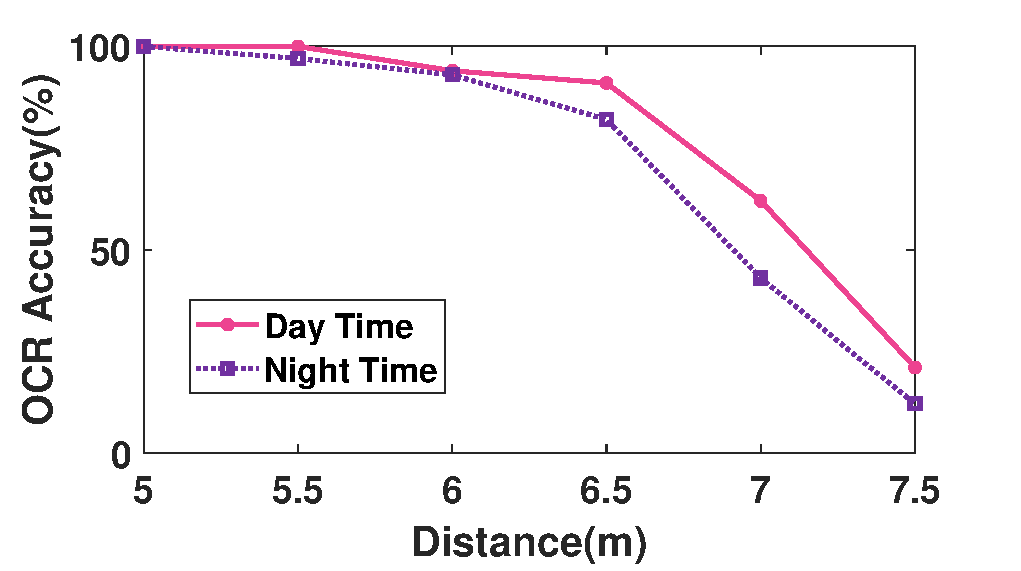
\includegraphics[width=0.24\textwidth]{./pic/data_1_2.pdf}\label{fig-control-2}}
    \subfigure[Traditional Lens]{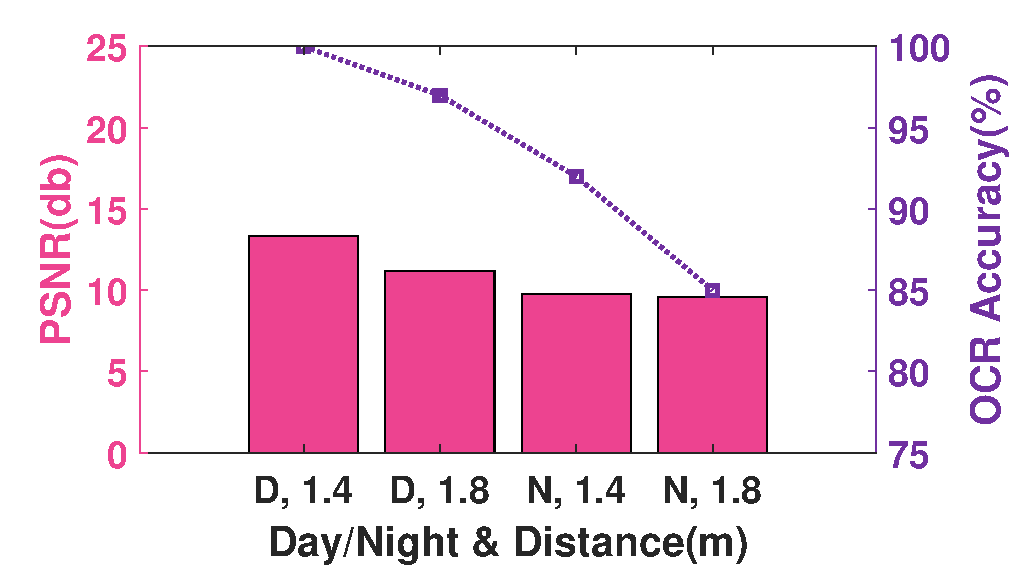
\includegraphics[width=0.24\textwidth]{./pic/data_2.pdf}\label{fig-random-1}}
    \subfigure[Optical Lens]{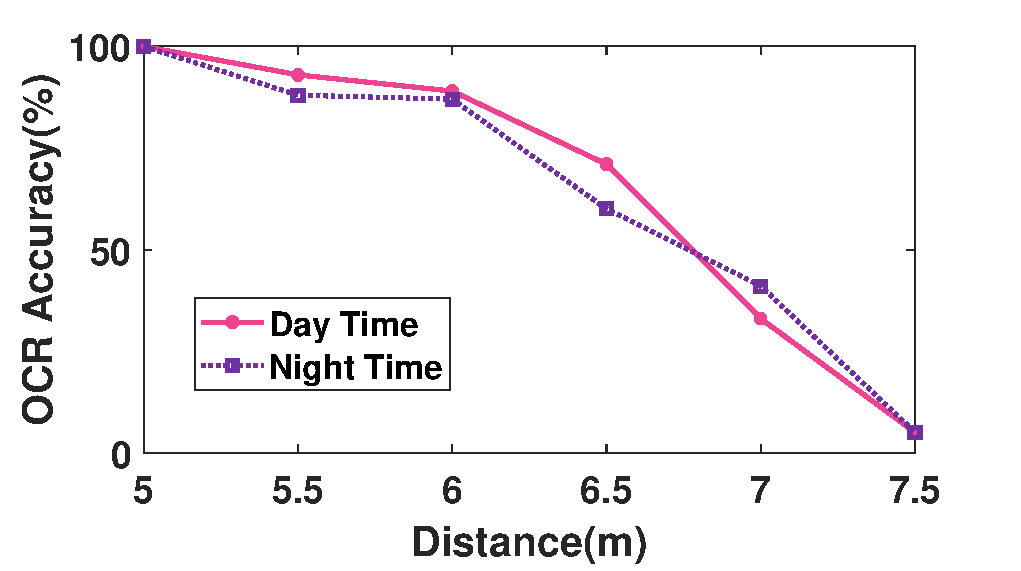
\includegraphics[width=0.24\textwidth]{./pic/data_2_2.pdf}\label{fig-random-2}}
    \hfill
    \caption{Performance in (a)(b). the random as well as (c)(d). the controlled environment using traditional lens and optical lens.}
    \label{fig:control_random}
\end{figure*}


\subsection{Performance with fewer available images}
As mentioned in sec.~\ref{sec-design}, our model is designed to work on any number of input images, the only limitation being that these images are snapshots of the same scene. This design is requisite because in certain scenarios the data displayed on the victim's screen is transient and ever-changing, e.g. password entry, where only the last character of the password is visible. We evaluated the impact of fewer available images to the performance of the SR model. The results are shown in fig.~\ref{fig:number_adapting}. We tested at the 1.8m daytime scenario for traditional lens and 6m daytime scenario for optical lens.

In the tradition lens group the performance of the model drops dramatically with fewer than 10 images, indicating that not enough input information is available to rule out all possibilities of the displayed characters. The optical lens group displayed a steady decent of accuracy when fewer images are available, which is expected, as the blur patterns are more complex and the differences between frames more pronounced, so that the images are more precious to the model and contain less overlapping data, and removing any of them will cause losses in accuracy.
\begin{figure*}[!t]
    \centering
    \subfigure[Traditional Lens]{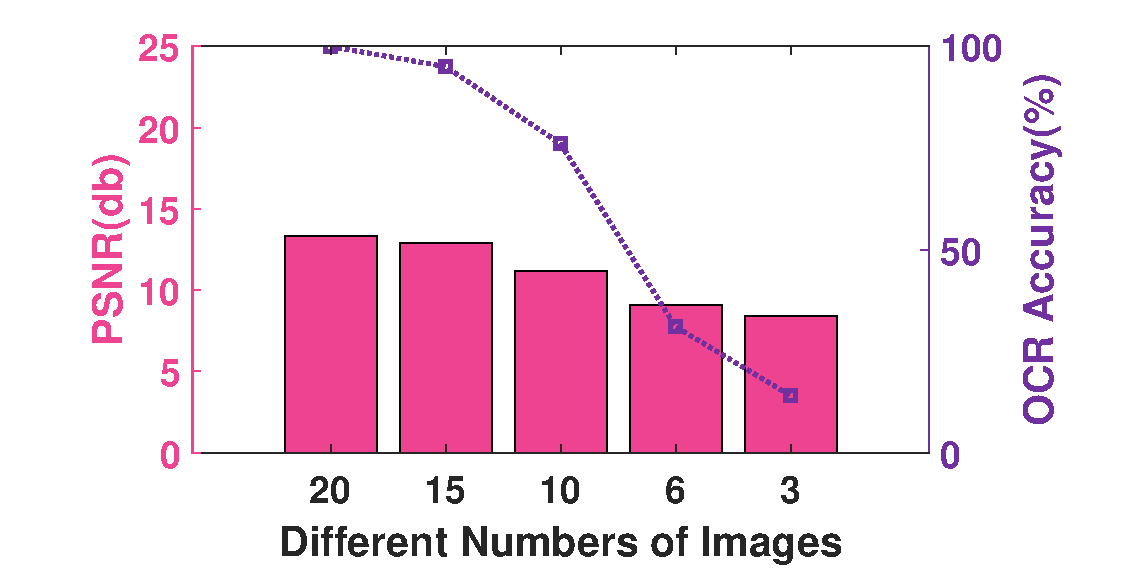
\includegraphics[width=0.24\textwidth]{./pic/data_5.pdf}\label{fig-image-tranditional-2}}
    \subfigure[Optical Lens]{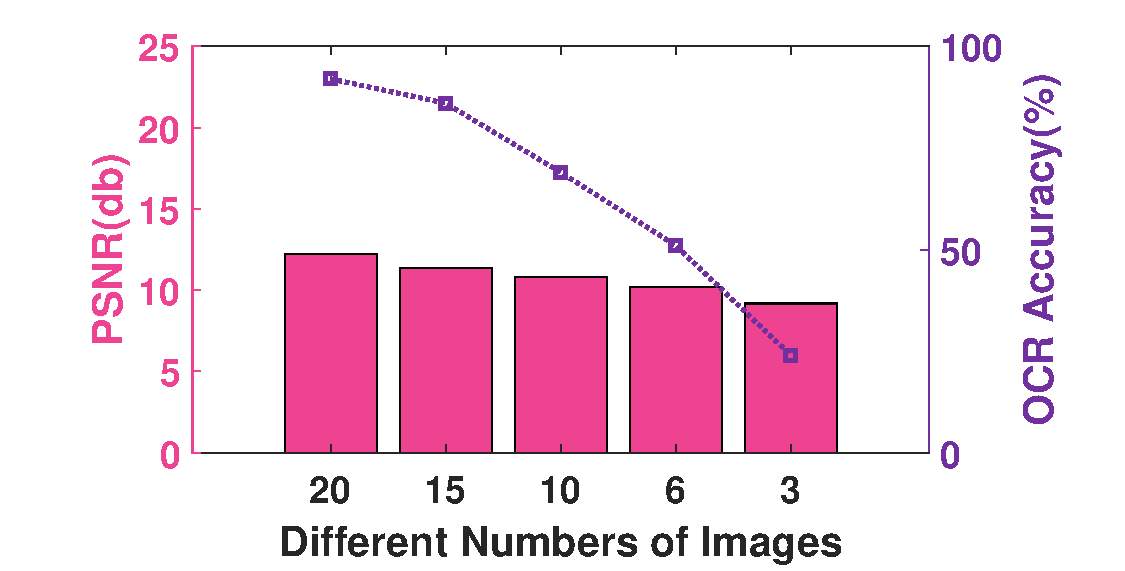
\includegraphics[width=0.24\textwidth]{./pic/data_6.pdf}\label{fig-image-optical-2}}
    \subfigure[Traditional Lens]{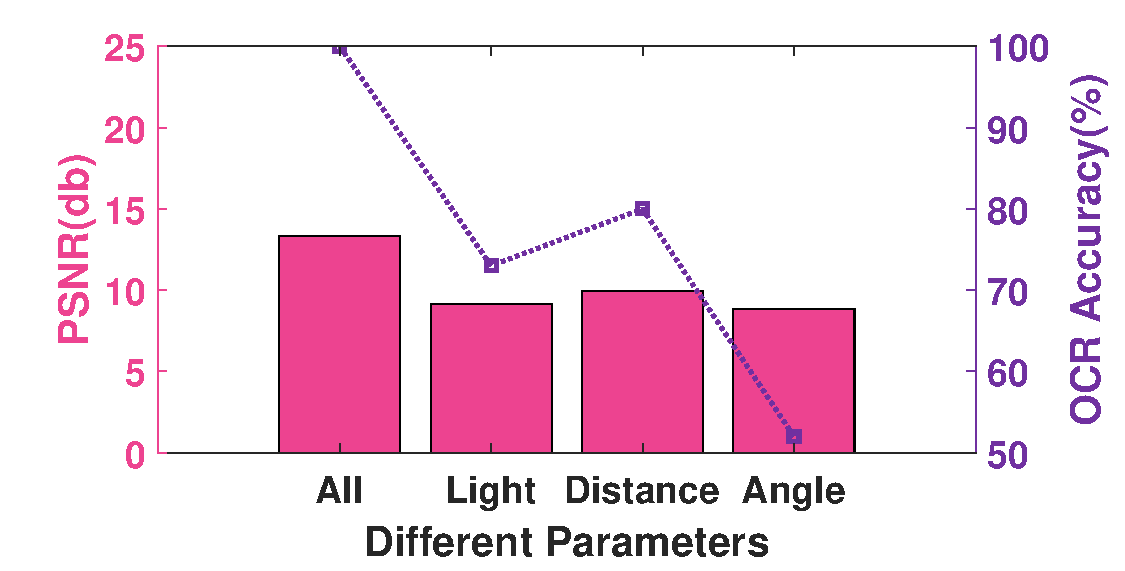
\includegraphics[width=0.24\textwidth]{./pic/data_3.pdf}\label{fig-adapt-tranditional}}
    \subfigure[Optical Lens]{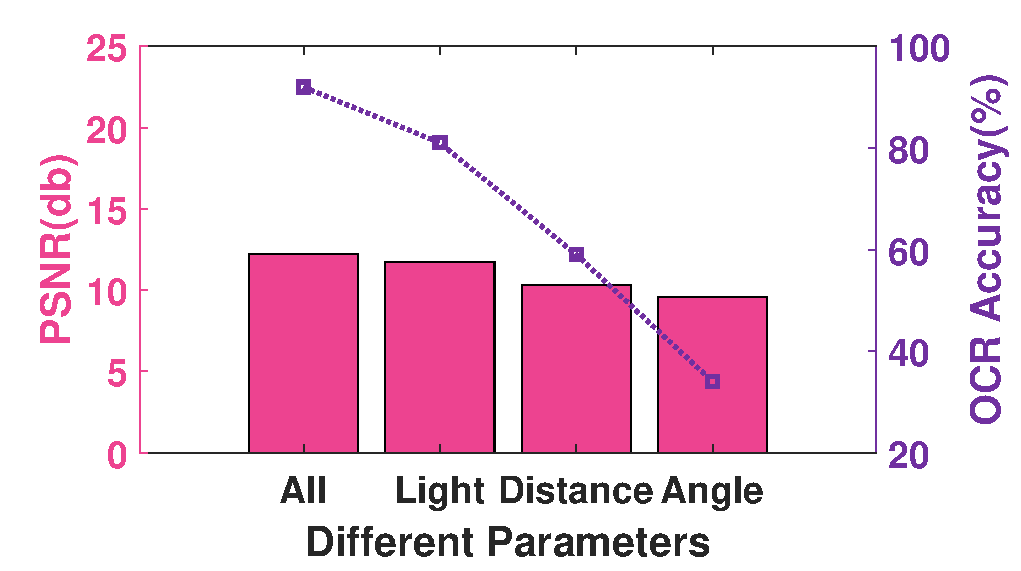
\includegraphics[width=0.24\textwidth]{./pic/data_4.pdf}\label{fig-adapt-optical}}
    \hfill
    \caption{Performance (a)(b). with fewer available images and (c)(d). for the adapting ability via traditional lens and optical lens.}
    \label{fig:number_adapting}
\end{figure*}

% \begin{figure}[!t]
%     \centering
%     \subfigure[Traditional Lens]{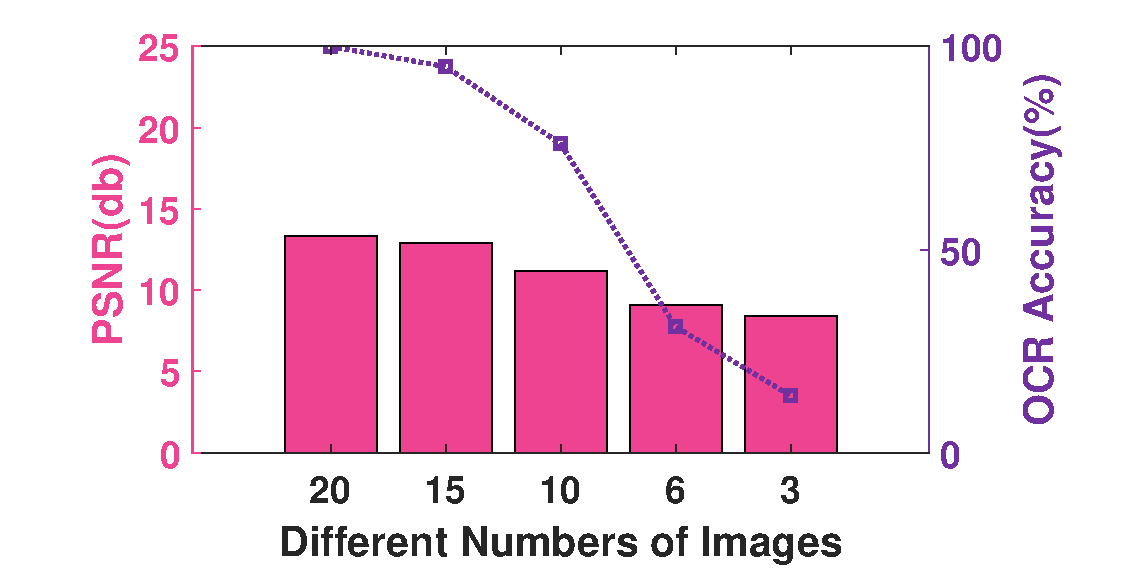
\includegraphics[width=0.40\textwidth]{./pic/data_5.pdf}\label{fig-image-tranditional-2}}
%     \subfigure[Optical Lens]{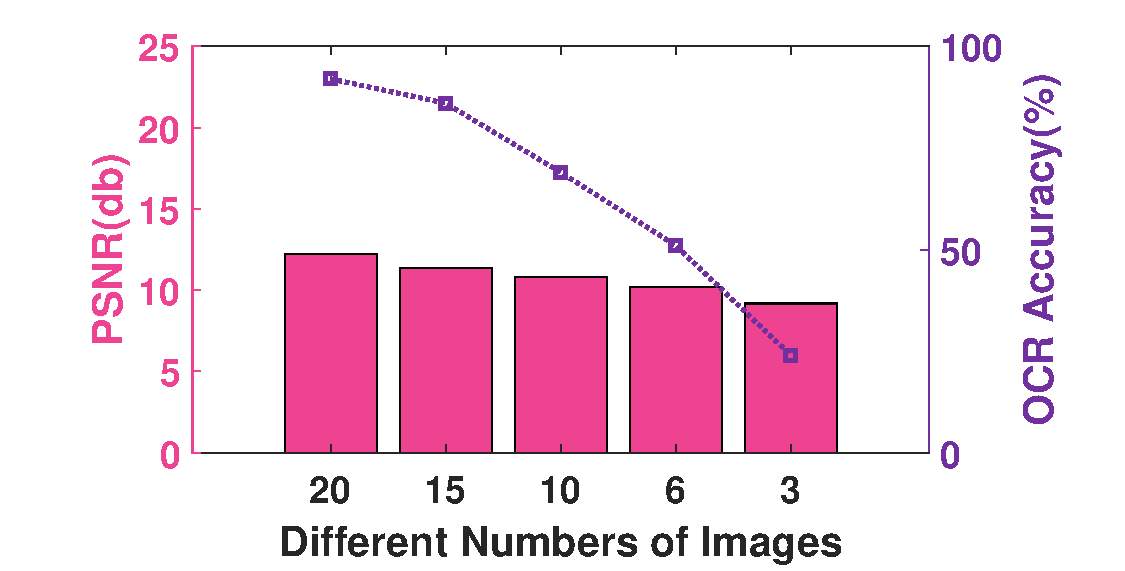
\includegraphics[width=0.40\textwidth]{./pic/data_6.pdf}\label{fig-image-optical-2}}
%     \hfill
%     \caption{Performance with fewer available images using traditional lens and optical lens.}
%     \label{fig:number}
% \end{figure}

\subsection{Adapting Ability}
We train the model with fewer groups of data, exposing it to fewer variations of environment parameters, and examine the model's performance in other environments. The results are shown in Figure~\ref{fig:number_adapting}.

We observed that variations in light and angle parameter in training data is crucial to a robust model. In the tradition lens group, the variations within 1 and 2 meters may have a smaller impact to the size of the characters
 so that features extracted at one distance might still exist at another.
 However, tilts and angles cause rotations and deformations and severely disturb the feature extraction process. The optical lens group yields similar results except at variations in distance. At a range of 6 meters, increases in distance leads to greater complexity of image blurriness, leading to more complex feature extraction and a more fragile model.
% \begin{figure}[!t]
%     \centering
%     \subfigure[Traditional Lens]{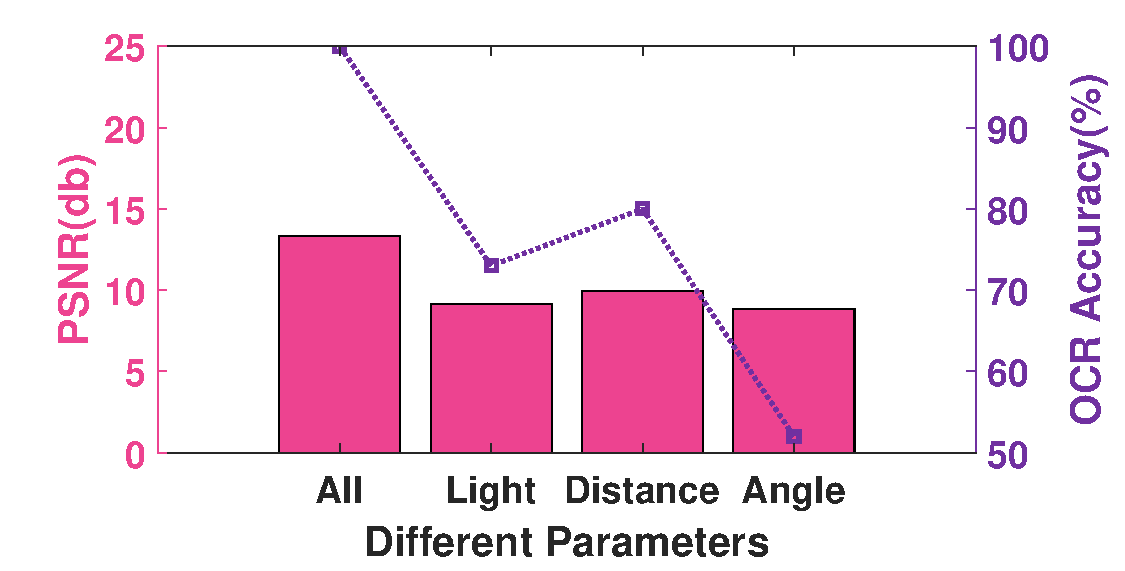
\includegraphics[width=0.40\textwidth]{./pic/data_3.pdf}\label{fig-adapt-tranditional}}
%     \subfigure[Optical Lens]{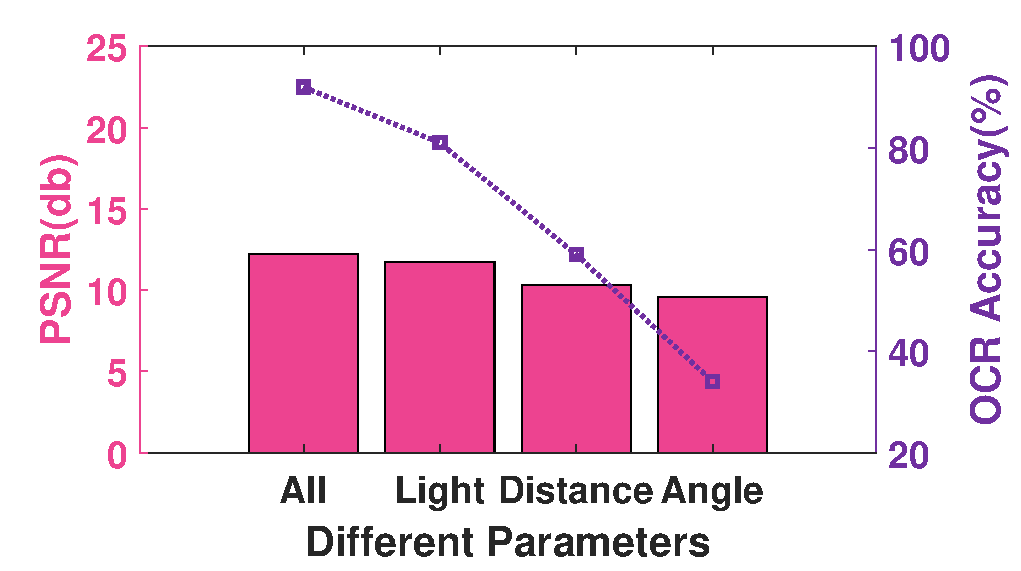
\includegraphics[width=0.40\textwidth]{./pic/data_4.pdf}\label{fig-adapt-optical}}
%     \hfill
%     \caption{Performance for the adapting ability using traditional lens and optical lens.}
%     \label{fig:adapting}
% \end{figure}

\subsection{Comparison with other architectures}
We train and test other widely used networks with the same sets of data and evaluate their results. We chose SRCNN, a commonly used single image SR network, applying it to each single image before merging the results by pixel-level average. We also used a multi-frame version of CNN consisting of 3D convolutional layers, designed for video super resolution (VideoSR). However, as mentioned above, it is very difficult for the single image approaches to utilize information and distinguish the noisy and deformed patterns, while VideoSR approaches rely upon consistency between frames, so they fail to give satisfactory results. We used the relatively easy 'daytime 1.2m-distance direct with traditional lens' group of data for testing. The results are shown in Table~\ref{table-comp}.
\begin{table}[!t]
    \centering
    \caption{Comparison with existing systems.}
    \begin{tabular}{@{}cccc@{}}
        \toprule
    System & SRPeek & SRCNN & VideoSR \\ \midrule
    PSNR & 13.32db & 7.69db & 8.403db\\ 
    OCR Accuracy & 100\% & 10\% & 23\%\\ \bottomrule
    \end{tabular}
    \label{table-comp}
\end{table}

We can see that the PSNR of SRPeek is 13.32dB which 73.2\% and 58.6\% larger than that of SRCNN and VideoSR. For the OCR accuracy, SRPeek can recognize all characters, but SRCNN and VideoSR can only recognize 10\% and 23\% of them. The results show the efficiency of our SR model in comparison with existing models.

% \section{System Evaluation}
\section{Case Study}
\label{case-study}
\subsection{Accuracy}

We build the system on smartphone and evaluate its performance in real-life scenarios (shown in Fig.~\ref{fig-reallife}). We experiment with a Redmi 6A smartphone (with a camera of 13 million pixels, no optical zooming) for the attacker and a HUAWEI Mate8 smartphone for the victim, with the former ``1.8m daytime'' setting. We ask 5 human participants to read the reconstructed characters to evaluate the usability of our model. No participants can read the unprocessed images, but all of them can decipher the information on the reconstructed image without much difficulty. The results are shown in Table~\ref{table-scenarios}.
\begin{figure}
	\centering
	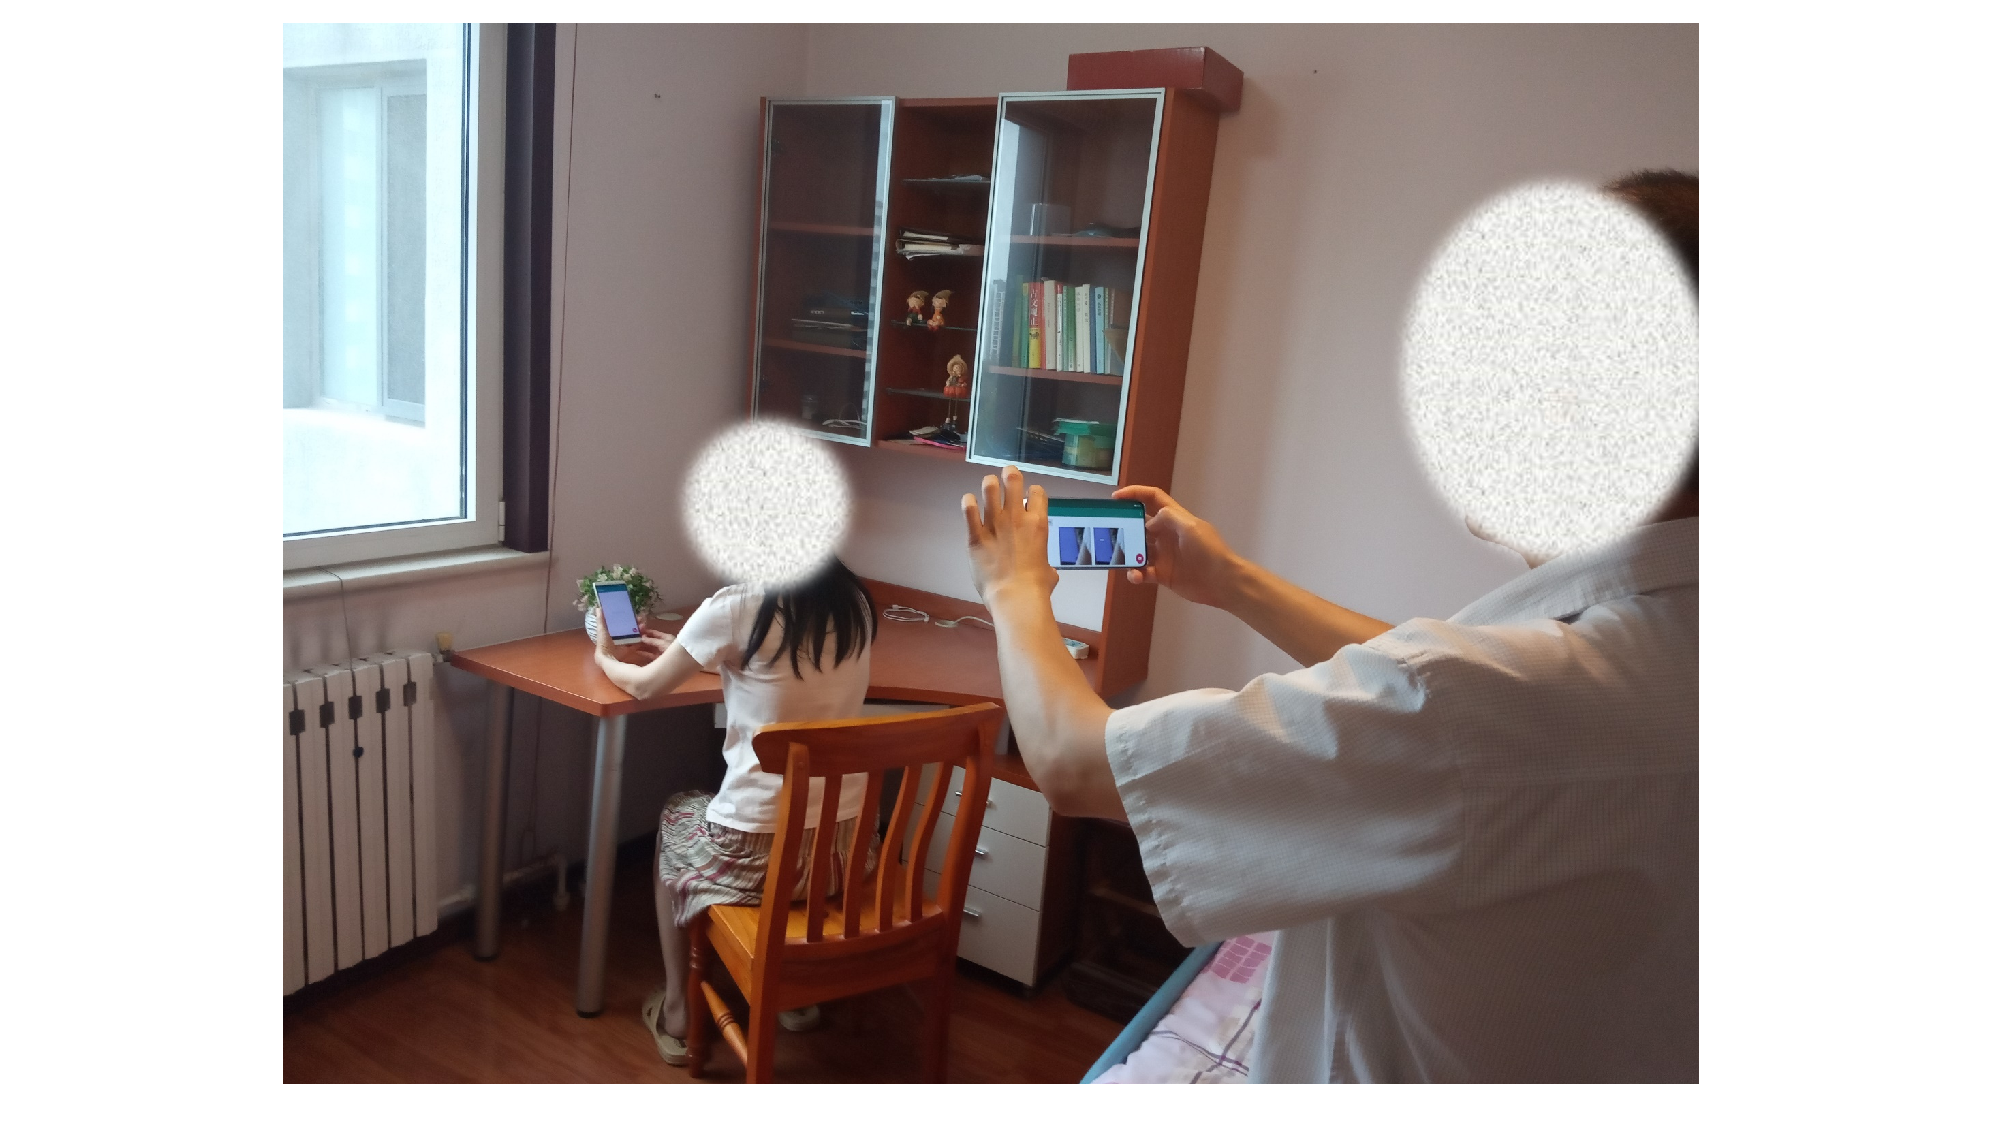
\includegraphics[width=0.80\linewidth]{pic/reallife.pdf}
    \caption{Illustration of our real-life scenario (Distance between attacker and victim is shortened for demonstration).}
	\label{fig-reallife}
\end{figure}

The results show that Human can read 95\%, 85\% and 70\% contents in home, transport and theater while the OCR accuracy is 100\%, 10\% and 23\%. That verifies human can obtain the most parts of information from the peeking in various environments. In transport, the vibration of smartphone and the darker environment can fool the OCR model for content recognition in comparison with human recognition so that leads lower accuracy in transport and theater.

\begin{table}[!t]
    \centering
    \caption{Recognition accuracy in various scenarios.}
    \begin{tabular}{@{}cccc@{}}
        \toprule
    Scenarios & Home & Transport & Theater \\ \midrule
    Baseline & 5\% & 0 & 0\\ 
    \midrule
    OCR & 100\% & 10\% & 23\%\\ 
    Human & 95\% & 85\% & 70\%\\ \bottomrule
    \end{tabular}
    \label{table-scenarios}
\end{table}

\subsection{Influence of hand tremors}
We ask 5 participants to capture images with handheld smartphones, keeping their hand still to their greatest effort (Handheld camera). We process these images and let them read the results. We compare this performance to the data collected on stationary phones to evaluate the influence of hand tremors.
We also ask participants to hold a smartphone in their hands and read a piece of text, without other additional instructions (Handheld target). The user may freely interact with the phone when reading. We capture images of the phone at the same time to see how our system deal with a moving target screen. The results are shown in Table~\ref{table-tremor}.

\begin{table}[!t] 
    \centering
    \caption{Impact of hand tremors when the camera (attacker phone) and/or target (victim phone) is handheld.}
    \begin{tabular}{ccccc}
        \toprule
    Accuracy & None & Camera & Target & Both  \\
    \midrule
    Baseline & 5\% & 0 & 5\% & 5\%\\ 
    \midrule
    OCR & 95\% & 85\% & 80\% & 80\%\\ 
    Human & 95\% & 85\% & 80\% & 85\%\\ \bottomrule
    \end{tabular}
    \label{table-tremor}
\end{table}

We can see that with the existence of tremors, the recognition accuracy drops from 95\% to 85\%/80\% for both OCR tools and human. We conclude from the results that hand tremors can impact the performance of our system. Hand tremors can cause motion blur and erratic shifts in the sub-pixel level(after image alignment phase) and impact performance.


\subsection{Success rate in different tasks}
We test the success rate of obtaining crucial information when the observed participant performs several tasks on a phone: reading text message, typing text message, entering PIN, and typing password with numbers, English and special characters(typing at 2 characters per second). We use accuracy per character as evaluation metric. In the PIN and password tasks, fewer photos will be available, but deciphering English characters is also easier than Chinese characters, and we use specifically trained models(with same structure and different training data). The results are shown in Table~\ref{table-task}.

\begin{table}[!t]
\centering
\caption{Success rate in different tasks.}
\label{table-task}
\begin{tabular}{@{}ccccc@{}}
	\toprule
Accuracy & Read text & Type text & Enter PIN & Enter password\\ \midrule
Raw Image & 5\% & 0 & 0 & 0\\
SRPeek & 100\% & 100\% & 100\% & 80\%\\ \bottomrule
\end{tabular}

\end{table}

We conclude that \textsf{SRPeek} functions normally in everyday scenarios and poses a threat to screen privacy.

\subsection{Perceived shoulder surfing susceptibility}
We ask the participants to rate the perceived shoulder-surfing susceptibility after the experiment. The attacker sits or stands at 1.8m range, pretending to be interacting with their own phone while continuously running the shoulder-surfing APP. None of the participants reported suspicion of shoulder-surfing. We believe that our system can enable a malicious attacker to gather large amounts of critical information from the victim while remaining unnoticed.






\section{Limitations \& Discussions}
\label{sec-limitations-and-discussions}
There are certain limitations of this work. We require a certain degree of image capturing and processing abilities of the attacker's phone, and we also expect the victim not to exert too much disturbance to the target phone.
\vspace{1mm}
\noindent
\textbf{Image Capturing Ability}
Latest models of smartphones can capture images at 10 frames per second in burst mode easily, however, this ability is not common in phones that are 3 years old. Heavily used phones also performs less than ideal when capturing images in burst mode. Also, when capturing images the user need to hold their phone as still as possible to avoid motion blur and assist image alignment. The user also has to keep a sharp focus on the target phone.

\vspace{1mm}
\noindent
\textbf{Processing Ability}
To achieve best performance the user needs a phone with strong processing capabilities to run the neural network at real time. As neural networks have been common place in numerous modern APPs, most phones of the latest generation have upgraded their processing ability to run neural networks, but older versions might not possess such processing powers and cannot process images at real-time.

\vspace{1mm}
\noindent
\textbf{Motion and Tremors}
In our experiment we assume the observed user will hold still his/hers phone, and not making interactions too often. However some users may tilt their phones during interactions—especially when typing with one hand. Too much tremor will cause motion blur in captured images and misalignment between frames, thus degrading the result.

Although our shoulder surfing system proves to be highly efficient against unprotected screens, there are some simple methods to mitigate this unique threat while not cumbering the user.

\vspace{1mm}
\noindent
\textbf{Dynamic background.} Most multi-frame SR algorithms are designed based on the assumption that all input images are reflections of the same scene, and ours is not an exception. By deploying a dynamic background behind the characters, such as tiny dots and lines travelling slowly around the screen, we can construct a constantly changing scene that will confuse the multi-frame SR algorithms, and due to the blurriness of the images, these influential elements cannot be easily removed. These dots do not need to be distinct or colored same as the the texts, as multi-frame SR algorithms function with tiny,pixel level differences between frames, making them especially sensitive to microscopic changes.

\vspace{1mm}
\noindent
\textbf{Active scanning.} There are several works providing an active countermeasure against shoulder surfing threats with the naked eye. With front-facing cameras and face detection algorithms, the smartphone can constantly scan the surrounding passers-by and detect their gaze direction, and give a warning to the user when that gaze points at the screen. However, to the extent of our knowledge none of these works have included cameras into their detection scope, but we believe it's practical to implement such features.

\vspace{1mm}
\noindent
\textbf{Adversarial machine learning methods.} In recent years we have discovered the weaknesses of neural networks and that inserting certain microscopic changes, undetectable to the human eye, to the pixels of an image will make it look different to a neural network. These methods fools the feature extraction phases of neural networks, so that SRPeek is also vulnerable to this attack. Theoretically, by exerting a pattern to the victim's screen, it can be captured by the attacker's camera and confuse its SR algorithms, but these remains to be implemented in our future work.

\section{Conclusion}
\label{sec-conclusion}
In this work we designed a holistic system, SRPeek, for shoulder surfing on smartphone, which serves as an up-to-date version of a threat model for shoulder surfing, and proved its efficiency. We proved that this threat towards screen privacy is imminent and can steal critical information, including personal texts or passwords, from long distances, thus escaping detection. It is our wish that this work can stur discussion in the field of screen privacy protection and proporgate defense mechanisms across critical mobile apps.

The core of SRPeek is a specially designed multi-frame SR network. With its innovative architecture this network outperforms other algorithms of the same field in our application. The design ideology enables this network to process higher levels of data integration ability while keeping a low calculation profile, and we believe the elements of this design can be used in other applications with large amounts of data, such as natural language processing or anomaly detection. Our model can also be used in OCR tasks when multiple images are avaliable, functioning as a preprocessor to improve the quality of the images and increase accuracy.
%\label{sec-conclusion}


%\clearpage

\bibliographystyle{abbrv}
\bibliography{main}

\end{document}


